%% 
%% Copyright 2007-2024 Elsevier Ltd
%% 
%% This file is part of the 'Elsarticle Bundle'.
%% ---------------------------------------------
%% 
%% It may be distributed under the conditions of the LaTeX Project Public
%% License, either version 1.3 of this license or (at your option) any
%% later version.  The latest version of this license is in
%%    http://www.latex-project.org/lppl.txt
%% and version 1.3 or later is part of all distributions of LaTeX
%% version 1999/12/01 or later.
%% 
%% The list of all files belonging to the 'Elsarticle Bundle' is
%% given in the file `manifest.txt'.
%% 
%% Template article for Elsevier's document class `elsarticle'
%% with numbered style bibliographic references
%% SP 2008/03/01
%% $Id: elsarticle-template-num.tex 249 2024-04-06 10:51:24Z rishi $
%%
\documentclass[preprint,12pt]{elsarticle}

%% Use the option review to obtain double line spacing
%% \documentclass[authoryear,preprint,review,12pt]{elsarticle}

%% Use the options 1p,twocolumn; 3p; 3p,twocolumn; 5p; or 5p,twocolumn
%% for a journal layout:
%% \documentclass[final,1p,times]{elsarticle}
%% \documentclass[final,1p,times,twocolumn]{elsarticle}
%% \documentclass[final,3p,times]{elsarticle}
%% \documentclass[final,3p,times,twocolumn]{elsarticle}
%% \documentclass[final,5p,times]{elsarticle}
%% \documentclass[final,5p,times,twocolumn]{elsarticle}

%% For including figures, graphicx.sty has been loaded in
%% elsarticle.cls. If you prefer to use the old commands
%% please give \usepackage{epsfig}

%% The amssymb package provides various useful mathematical symbols
\usepackage{amssymb}
%% The amsmath package provides various useful equation environments.
\usepackage{amsmath}
%% The amsthm package provides extended theorem environments
%% \usepackage{amsthm}

%% The lineno packages adds line numbers. Start line numbering with
%% \begin{linenumbers}, end it with \end{linenumbers}. Or switch it on
%% for the whole article with \linenumbers.
%% \usepackage{lineno}

\newcommand\hmmax{0}
\newcommand\bmmax{0}
\usepackage[T1]{fontenc} 
\usepackage[utf8]{inputenc}
\usepackage{amsmath}
\usepackage{amsthm}
\usepackage{amsfonts}
\usepackage{amssymb}
\usepackage{mathrsfs}
\usepackage{anyfontsize}
\usepackage{mdframed}
\usepackage{tikz}
\usepackage{verbatim}
\usepackage{booktabs}
\usepackage{array}
\usepackage{enumitem}
\usepackage{bbold}
\usepackage{fancyhdr}
\usepackage{blindtext}
\usepackage[top=1in, bottom=1.5in, left=1in, right=1in]{geometry}

\usepackage{MnSymbol}

\usepackage[cal=boondox,scr=boondoxo]{mathalfa}

\usepackage{float}
\usepackage{adjustbox}
\usepackage{subfig}
\usepackage{fancybox,graphicx}
\usepackage{caption}
\usepackage{color}
\usepackage{amsmath}  
\usepackage{stmaryrd}  
\usepackage{bm}  
\usepackage{bbm}
\usepackage{hyperref} % pour les liens hypertextes
\usepackage{cleveref}
\usepackage{setspace}

% DOI and ARXIV Commands for Bib Files
% Written by Daniel Herber
% -----------------------------------------------
% one option is to use the 'note' field with this command
% -----------------------------------------------
% for example, if your doi is 10.2514/1.J052182
% then for the citation for the reference in your bib file, use
% note = "\doi{10.2514/1.J052182}",
% -----------------------------------------------
% for example, if your arxiv number is 0706.1234
% then for the citation for the reference in your bib file, use
% note = "\arxiv{0706.1234}",

% requires hyperref package for \href command
\usepackage{hyperref}

% doi command (use in bib file)
\newcommand{\doi}[1]{{doi:~\href{https://doi.org/#1}{\nolinkurl{#1}}}\rmFullStop}

% arXiv command (use in bib file)
\newcommand{\arxiv}[1]{{arXiv:\href{https://arxiv.org/abs/#1}{#1}}\rmFullStop}

% command to remove full stop if the next character
\newcommand*{\rmFullStop}{\rmifnextchar{.}{}{}}

% command to check the next character and replace if present
% \rmifnextchar{X}{[removed text]}{[no X text]}
% if X is the next character, then it is removed and [removed text] is inserted
% otherwise, the character is not removed and [no X text] is inserted
% based on http://tex.stackexchange.com/questions/72827
\makeatletter
\newcommand{\rmifnextchar}[3]{%
  \begingroup
  \ltx@LocToksA{\endgroup#2}%
  \ltx@LocToksB{\endgroup#3}%
  \ltx@ifnextchar{#1}{%
    \def\next{\the\ltx@LocToksA}%
    \afterassignment\next
    \let\scratch= %
  }{%
    \the\ltx@LocToksB
  }%
}
\makeatother %doi command

\usepackage{accents}
\usepackage[titletoc,title]{appendix}


%floor and ceiling functions
\usepackage{mathtools}
\newcommand{\soft}{\mathcal{S}}
\newcommand{\hard}{\mathcal{H}}
\newcommand*\underdot[1]{ \underaccent{\bullet}{\mathcal{#1}} } %requiere: \usepackage{accents} 
\newcommand*\UnderDot[1]{ \underaccent{\bullet}{#1} } %requiere: \usepackage{accents} 

\usepackage{stackengine}
\newcommand\barbelow[1]{\stackunder[2.5pt]{$#1$}{\rule{1.2ex}{.15ex}}}

\newcommand{\pvec}[1]{\vec{#1}\mkern2mu\vphantom{#1}} %to prime a vector

\newcommand*\UnderTilde[1]{ \underaccent{\sim}{#1} }
  
\renewcommand{\figurename}{Fig.}
\journal{Nuclear Physics B}
\journal{Magnetic Resonance Imaging}

\newtheorem{theorem}{Proposition}
\renewcommand{\qedsymbol}{}
\newcommand{\parallelsum}{\mathbin{\!/\mkern-5mu/\!}}

\begin{document}

\title{Rapport de stage sur l'analyse de données d'IRM par régression logistique multivoie multibloc} %% Article title

%% use optional labels to link authors explicitly to addresses:
%% \author[label1,label2]{}
%% \affiliation[label1]{organization={},
%%             addressline={},
%%             city={},
%%             postcode={},
%%             state={},
%%             country={}}
%%
%% \affiliation[label2]{organization={},
%%             addressline={},
%%             city={},
%%             postcode={},
%%             state={},
%%             country={}}

\author{Alexandre SELVESTREL} %% Author name

%% Author affiliation
\affiliation{organization={Laboratoire des systèmes, Centrale-Supélec},%Department and Organization
            addressline={}, 
            city={Orsay},
            postcode={}, 
            state={Paris},
            country={France}}

            \begin{center}
              \vspace*{4cm}
              \setstretch{2} % Augmenter l'interligne
              {\LARGE \textbf{Rapport de stage de fin d'études sur l'analyse par machine learning de données médicales multivariées}} \\[5em]
              {\large Alexandre SELVESTREL}\\[1em]
              {\large Laboratoire des systèmes, Centrale-Supélec}\\[1em]
              {\large Encadrants: Arthur Tenenhaus, Laurent Lebrusquet}\\
              \vspace*{\fill}
              Soutenance le 29 Novembre 2024
          \end{center}

\newpage

\section*{Synthèse (version française)}
\paragraph*{Présentation générale} L'objectif de mon stage était de réaliser une classification automatique (via du machine learning) de tumeurs du foie basée sur des IRMs et sur quelques données cliniques (âge, sexe du patient ...). Cette classification devait permettre de tester et améliorer des modèles tensoriels récents \cite{multi_rank_1,multi_rank_r} et de vérifier si ceux-ci donnaient de meilleures performances que les autres modèles. Ce stage était effectué au laboratoire des systèmes (l2S) en partenariat avec l'assistance publique des hôpitaux de Paris (AP-HP). Sur le versan médical, nous avons pu bénéficier de l'aide de Sébastien Mulé, Maître de conférence à la faculté de santé, Université Paris-Est Créteil (UPEC) et Radiologie, chef du département imagerie de l'hôpital Henri Mondor.

\paragraph*{Enjeux} Ce stage s'inscrit dans la cadre de la collaboration entre le l2S et l'AP-HP. Du point de vue du l2S, il s'agit de mettre à l'épreuve des méthodes de machine learning particulières, basées sur des tenseurs et qui semblent spécifiquement adaptées aux données étudiées. Par ailleurs, en me formant au machine learning appliqué au domaine médical, le laboratoire s'assure dès le début du stage qu'en poursuivant en doctorat, je disposerai des compétences nécessaires pour être immédiatement opérationnel.\\
\indent Pour l'AP-HP, l'enjeu est de faire progresser la recherche sur le cancer du foie. En effet, la détermination de la nature de la tumeur du foie d'un patient est un problème complexe auquel il n'existe pas de solution complètement satisfaisante à l'heure actuelle. Or, les médecins disposant des IRMs des patients malades, il serait dommage de ne pas les utiliser pour tenter de proposer un outil de diagnostic automatique. Même dans le cas où cet outil serait moins performant que ce qui existe déjà, il pourraît être utile aux médecins pour déterminer de nouveaux indices qui caractérisent la classe d'une tumeur.

\paragraph*{Solutions et résultats:} Nous avons commencé par implémenter des modèles statistiques basiques (régression logistique lasso et random forest) sur les données de cancer du foie. Cela nous a permis d'établir une valeur de référence pour la performance de la classification (AUC = 0.68). Nous avons ensuite cherché à améliorer ce score en prorammant une régression logistique tensorielle (voir la section "Méthodes"). Mais malgré plusieurs tentatives d'amélioration du modèle (notamment en séparant les variables en plusieurs blocs), aucun gain de performance n'était observé.\\
\indent Afin de vérifier que notre modèle était pertinent, nous avons alors cherché à tester son efficacité sur des données simulées. Sur ces données, notre modèle tensoriel a montré des performances bien meilleures que les modèles non tensoriels. Cela nous a permis de conclure que ce modèle était pertinent dans certains cas et que le manque de performance observé sur les données médicales était probablement dû à la mauvaise qualité de ces données.\\
\indent Après plus d'un mois de trvail pour améliorer la qualité des données, je me suis rendu à l'Hôpital Henri Mondor afin d'en parler avec Sébastien Mulé sur son lieu de travail (et non dans mon laboratoire comme les fois précédente). Cela a permis de découvrir l'existence d'un autre jeu de données complètement ommises jusqu'à présent, beaucoup plus simples (seulement une quinzaine variables par individu), donnant des résultats bien meilleures que les données précédentes quand on les traite par machine learning. Nous avons été un peu pris de court par l'arrivée au dernier moment de ces données qui, bien que de bonne qualité, ne sont pas adaptées aux modèles tensoriels. Nous ne les mentionnons donc pas dans la partie "article" du rapport mais nous les présentons juste après.\\

\newpage
\tableofcontents
\newpage



\begin{frontmatter}

  
%% Title, authors and addresses

%% use the tnoteref command within \title for footnotes;
%% use the tnotetext command for theassociated footnote;
%% use the fnref command within \author or \affiliation for footnotes;
%% use the fntext command for theassociated footnote;
%% use the corref command within \author for corresponding author footnotes;
%% use the cortext command for theassociated footnote;
%% use the ead command for the email address,
%% and the form \ead[url] for the home page:
%% \title{Title\tnoteref{label1}}
%% \tnotetext[label1]{}
%% \author{Name\corref{cor1}\fnref{label2}}
%% \ead{email address}
%% \ead[url]{home page}
%% \fntext[label2]{}
%% \cortext[cor1]{}
%% \affiliation{organization={},
%%            addressline={}, 
%%            city={},
%%            postcode={}, 
%%            state={},
%%            country={}}
%% \fntext[label3]{}


%% Abstract
\begin{abstract}
%% Text of abstract
Abstract text.
\end{abstract}

% %%Graphical abstract
% \begin{graphicalabstract}
% %\includegraphics{grabs}
% \end{graphicalabstract}

% %%Research highlights
% \begin{highlights}
% \item Research highlight 1
% \item Research highlight 2
% \end{highlights}

%% Keywords
\begin{keyword}
  Machine Learning \sep tensor model \sep MRI 
%% keywords here, in the form: keyword \sep keyword

%% PACS codes here, in the form: \PACS code \sep code

%% MSC codes here, in the form: \MSC code \sep code
%% or \MSC[2008] code \sep code (2000 is the default)

\end{keyword}

\end{frontmatter}

%% Add \usepackage{lineno} before \begin{document} and uncomment 
%% following line to enable line numbers
%% \linenumbers

%% main text
%%

%% Use \section commands to start a section
\section{Introduction}
% Use \subsubsection, \paragraph, \subparagraph commands 
\indent Il existe deux grands types de tumeur du foie: les carcinome hépatocellulaire (CHC) et les cholangiocarcinomes (CCK). Certaines tumeurs présentent même des caractéristiques CCK et CHC selon l'endroit du foie observé et sont alors dites mixtes. Or, le traitement des tumeurs du foie dépendant de leur classe, il est important de savoir les distinguer efficacement. Pour l'instant, deux grandes approches existent: la microscopie et la radiographie avec injection de produit contrastant.\\
\indent La microscopie est la méthode la plus fiable car elle permet de directement analyser les cellules tumorales. Toutefois, puisqu'elle nécessite de prélever un petit morceau de foie cancéreux, elle demande une opération et peut entraîner des complications chez le patient. De plus, elle ne donne accès qu'à un fragment du foie, qui n'est pas nécessairement représentatif de l'ensemble de la tumeur. La radiographie (par IRM ou scanner) avec injection de produit contrastant est au contraire non invasive et donne accès à la tumeur en 3D dans son intégralité. À mesure que le produit de contraste se diffuse dans le foie, des images sont prises à quatre temps différents (artériel, portal, veineux et tardif) pour observer des caractéristiques spécifiques de chaque phase. Cependant, ces images ne permettent pas de déterminer à l'oeuil nu avec certitude la nature de la tumeur \cite{desaccord}. En effet, les caractéristiques des tumeurs CHC et CCK sont souvent très proches et les experts ne sont pas toujours d'accord entre eux lorsqu'ils analysent les images.\\
\indent Cet article tente de pallier les limites de l'analyse à l'oeuil nu par l'emploi de machine learning. Etant donné le fable nombre de patients étudiés (environ une centaine) et l'exigeance d'explicabilité liée au domaine médical, le machine learning classique est privilégié par rapport au deep learning. Par ailleurs, toujours à cause du faible nombre de patients et afin de simplifier l'étude, les tumeurs mixtes ne sont pas prises en compte. En effet, celles-ci sont encore mal comprises par les médecins, qui préfèrent même parfois les catégoriser comme CHC ou CCK selon l'aspect qui prédomine dans la tumeur.\\
\indent Les features de chaque tumeur sont extraites des images radiographiques à l'aide de la librairie Python pyradiomics \cite{pyradio}. Pour chaque patient, la tumeur est observée sur quatre images distinctes, prises à des moments spécifiques correspondant aux différentes phases d'acquisition (artérielle, portale, veineuse et tardive). Les mêmes variables sont donc mesurées pour chacune de ces phases. Ainsi, pour chaque patient, les features s'organisent selon une matrice de taille $J \times K$ où $J$ est le nombre de features extraites par pyradiomics dans chaque radio et $K$ est le nombre de phases d'acquisition. En empilant ces matrices les unes sur les autres, pour chaque individu, on forme un tenseur de taille $n \times J \times K$, où $n$ est le nombre d'individus étudiés: on parle donc de données tensorielles\\
Le modèle principal adopté dans cet article est une régression logistique avec pénalisation lasso, qui permet une sélection parcimonieuse des variables explicatives. Cette propriété est particulièrement utile pour traiter le grand nombre de caractéristiques extraites par pyradiomics. Afin de prendre en compte la structure tensorielle des données, plusieurs modèles spécifiques aux données tensorielles, présentés en section \ref{sec:models}, ont été étudiés. Ces modèles sont comparés au group lasso \cite{grp_lasso}, afin de vérifier si le simple regroupement des variables en paquets distincts peut suffire à capturer les relations pertinentes entre features (ou bien s'il est indispensable de tenir compte pleinement de l'aspect tensoriel des données pour obtenir les meilleurs résultats). \\




\section{Methodology}

\subsection{Tensorial data and notations}

% We will denote as a tensor any multidimensionnal array, i.e. $\underline{\mathbf{X}} = (x_{i_1i_2...i_m})_{i_1 \in \llbracket 1, I_1 \rrbracket, i_2 \in \llbracket 1, I_2 \rrbracket, ... i_M \in \llbracket 1, I_M \rrbracket}$. It is the extension of the matrix to any finite dimension. To avoid confusion with the notion of dimension of a vector space, and in line with the conventions promoted in Kolda and Bader \cite{conventions}, these dimensons will be referred to as "mode" in the following and their number will be referred to as the "order" of the tensor.\\
\indent We designate as tensorial data any data where the explanatory variables are structured along several dimensions. To avoid confusion with the notion of dimension of a vector space we call these dimensions modes in the following. For example, if like in our real data, we measure the same quantities at several fixed times and depths, we say that time and depth are modes in our data. Then, instead of having a matrix of explanatory variables $\mathbf{X} = (x_{ij})_{i \in \llbracket 1, n \rrbracket, j \in \llbracket 1, J \rrbracket}$ (where $i$ is the individual and $j$ is the quantity of interest), we get a tensor of explanatory variables $\underline{\mathbf{X}} = (x_{ijk_1k_2\text{ ... }k_M})_{i \in \llbracket 1, n \rrbracket, j \in \llbracket 1, J \rrbracket, k_1 \in \llbracket 1, K_1 \rrbracket \text{ ... } k_m \in\llbracket 1, K_M \rrbracket } $  (where $i$ is the individual, $j$ is the quantity of interest and where for $m \in \llbracket 1, M \rrbracket$, $k_m$ is the $k_m$-th modality of the $m$-th mode of the data). In terms of notations, we use those of Kolda and Bader \cite{conventions}, especially concerning matricization (see section 2.4 of \cite{conventions}). However, as some details need to be precised, we do this here:\\

\noindent $\bullet \; \;$ The concatenation of two matrices $\mathbf{A}$ and $\mathbf{B}$ by juxtaposing their columns side by side is denoted $[\mathbf{A} \; \; \mathbf{B}]$.\\
$\bullet \; \;$ To avoid overuse of the symbol $\phantom{a}^T$, we also define a notation to designate the juxtaposition of two matrices one below the other. Thus, the matrix defined by block with $\mathbf{A}$ above $\mathbf{B}$ is denoted $\left[\mathbf{A}; \, \mathbf{B}\right]$. It can also be written $[\mathbf{A}^T \; \; \mathbf{B}^T]^T$ but this multiplies the $\phantom{a}^T$ symbols, which impairs legibility. \\
$\bullet \; \;$ Since vectors are column matrices, using the same notation, we write the concatenation of two vectors $\mathbf{u}$ and $\mathbf{v}$ as follows: $[\mathbf{u}; \, \mathbf{v}]$.  \\
$\bullet \; \;$ The vector (column) whose elements are $(u_i)_{i \in \llbracket 1, I\rrbracket}$ is denoted $(u_1, u_2, \; \; \hdots \;\; u_I)$. \\
$\bullet \; \;$ If $\mathbf{X}$ is a matrix of explanatory variables, $\mathbf{x}_i$ is the vector (column) composed of the i-th row of $\mathbf{X}$.\\
$\bullet \; \;$ The vector of length $I$ filled with $1$ is denoted by $\mathbbm{1}_I$.\\
$\bullet \; \;$ We denote $\text{Diag}(\mathbf{u})$ the diagonal matrix whose diagonal is the vector $\mathbf{u}$. \\
% $\bullet \; \;$ For other notations, we use the conventions employed by Kolda and Bader \cite{conventions}. In particular, when we transform a tensor $\underline{\mathbf{X}}$ into a matrix (by unfolding it) using the first mode to form the rows, we do so as follows: $[\mathbf{X}_{:\,:1} \; \; \ldots \; \;\mathbf{X}_{:\,:K}]$ and we denote $\mathbf{X}_{(1)}$ the matrix thus obtained.

% \indent In order to train models that are not specific to tensor data (like a penalized logistic regression), we unfold the tensor $\underline{\mathbf{X}}$ and transform it into a matrix by placing each slice at a fixed $k$ next to the other. This gives the following matrix: $\mathbf{X}_{(1)} = [\mathbf{X}_{:\,:1}, \ldots, \mathbf{X}_{:\,:K}]$. However, in doing so, the model is no longer informed that $\underline{\mathbf{X}}$ is made up of the same quantities observed at different times. One of the reason for which this is important is that there is a non negligeable correlation between variables describing the same quantity of interest at different times. We'll still use the group lasso to restore this information to the model by grouping together variables belonging to the same time, but this is not enough to recover the full tensor aspect of the initial data. Furthermore, as pointed out by Le Brusquet et al. \cite{multi_rank_1}, unfolding the matrix greatly increases the number of predictors compared to tensor methods, which can increase computation times. However, given that in our dataset, $K$ is small ($K = 4$), this increase in computation time is not observed with our data.\\


\subsection{Machine learning models}
\label{sec:models}

In this section, we describe all the machine learning methods that we used and compared in order to get our results. We start briefly by non tensorial methods and then we describe in details the tensorial methods that we used. For the sake of simplicity, we only describe the situation where $\underline{\mathbf{X}}$ is a tensor of order 3. However, all the methods described here can be generalized to tensors of any order.
\subsubsection{Non tensorial methods}
For these methods, we start by unfolding the tensorial data $\underline{\mathbf{X}}$ into the matrix $\mathbf{X}_{(1)} = [\mathbf{X}_{:\,:1}\; \; \ldots \; \;\mathbf{X}_{:\,:K}]$. We then complete this matrix  by concatenating (along the columns) the matrix of non tensorial data $\mathbf{X}_{\text{tab}}$ (where "tab" stands for "tabular"). By doing so we obtain $\mathbf{X}_{\text{tot}} = [\mathbf{X}_{(1)} \; \; \mathbf{X}_{\text{tab}}]$.\\
\indent We first train a penalized logistic regression lasso on $\mathbf{X}_{\text{tot}}$. Then, still based on the matrix $\mathbf{X}_{\text{tot}}$, we train a group lasso \cite{grp_lasso}. In order to make a comparison with tensorial models, we group by variable name or by mode. When the data is structure according to variable blocs, we finally group by block. 
\subsubsection{Multiway logistic regression with lasso}
\indent We now turn to tensor approaches. We start by studying a multiway logistic regression penalized by lasso. This model is described for rank 1 in Le Brusquet et al. \cite{multi_rank_1} and in Girka et al. \cite{multi_rank_r} for its extension to rank $R \in \mathbb{N}^{*}$. In this report, we directly describe the generalization to rank $R \in \mathbb{N}^{*}$, rank $1$ being a special case of this model.\\[5 pt]

\noindent The fundamental idea of the model is to decompose the parameter $\bm{\beta}_{\text{tens}} \in \mathbb{R}^{JK}$ associated with the tensor explanatory variables of the logistic regression as:
\begin{equation}
    \bm{\beta}_{\text{tens}} = \sum\limits_{r = 1}^R\bm{\beta}_r^K \otimes \bm{\beta}_r^J
\end{equation}
with for all $r \in \llbracket 1 ,R \rrbracket$, $\bm{\beta}_r^J \in \mathbb{R}^J$ and $\bm{\beta}_r^K \in \mathbb{R}^K$. To take account of the $M$ tabular variables (non tensorial), we associate them with a coefficient $\bm{\beta}_{\text{tab}} \in \mathbb{R}^M$. In this way, the parameter $\bm{\beta}$ of the logistic regression is written: $\left[\bm{\beta_{\text{tens}}}; \, \bm{\beta_{\text{tab}}} \right]$.\\
As usual with logistic regressions, we consider that each realization of the explained variable $y_i$ ($i \in \llbracket 1, n \rrbracket$) follows an independent Bernoulli law conditionally on $\mathbf{x_i}$. For logistic regression, this proba is parametrzied by $\bm{\beta}$ and defined as
\begin{equation}
    \label{eqref:vraisemblance}
    \mathbb{P}( y_i = 1\, | \, \mathbf{x}_i) = \frac{1}{1 + \exp(- \mathbf{x}_i^T \bm{\beta} - \beta_0)}
\end{equation}
where  $\beta_0 \in \mathbb{R}$ is the intercept\\ %and $\mathbf{x}_i \in \mathbb{R}^{JK}$ is given by $\mathbf{x}_i = {(\mathbf{x}_{\text{tot}}})_{i:}$ \\

\noindent We set  $\bm{\beta}^J = \left[\bm{\beta}_1^J ; \;\; \hdots \; \; ;\,\bm{\beta}_R^J \right]$ and  $\bm{\beta}^K = \left[\bm{\beta}_1^K; \; \; \hdots \; \; ;\,\bm{\beta}_R^K \right]$.
\vspace{5 pt}
\noindent In order to simplify the calculations, while ensuring that the penalty continues to promote sparse models, we adapt the definition of the lasso penalty. The new penalty defines the following optimization problem: %\in \mathbb{R}\times \mathbb{R}^{RJ} \times  \mathbb{R}^{RK} \times \mathbb{R}^M
\begin{equation}
    \beta_0, \bm{\beta}^J, \bm{\beta}^K, \bm{\beta}_{\text{tab}} \; = \hspace{-8pt} \underset{\beta_0 ,\, \bm{\beta}^J, \, \bm{\beta}^K, \, \bm{\beta}_{\text{tab}}}{\text{argmin}} \left[ - \sum\limits_{i = 1}^{N} \log(\mathbb{P}(y_i = 1 \, | \mathbf{x}_i)) + \lambda \left(\sum\limits_{r = 1}^R
    \lVert \bm{\beta}_r^K \otimes \bm{\beta}_r^J \rVert_1 + \lVert \bm{\beta}_{\text{tab}} \rVert_1 \right)\right]
\end{equation}

\noindent Optimization is performed by alternating directions between $\left[ \beta_0 ;\, \bm{\beta}^J  ; \,  \bm{\beta}_{\text{tab}}   \right]$ and  $\left[ \beta_0; \, \bm{\beta}^K  ;\, \bm{\beta}_{\text{tab}}  \right]$. The stopping criterion is defined by the relative difference between the value of the objective function before optimization in the first direction and the value of the same function after optimization in the second direction.  We note that optimizing the loss function in each of these directions is tantamount to performing a simple logistic regression with a lasso penalty. Indeed, if we denote $C$ the loss function of classical logistic regression penalized by lasso (for any $K_0 \in \mathbb{N}^{*}$):

\begin{equation}
    %% Gerer l'allign
    C: \begin{cases}
        \begin{array}{ccl}
            \mathbb{R} \times \mathbb{R}^{K_0} \times \mathbb{R}^{N \times K_0} \times \mathbb{R}^{N} \times \mathbb{R} & \longrightarrow & \mathbb{R}                                                                                                                                                                    \\
            (\beta_0, \bm{\beta}, \mathbf{X}, \mathbf{y}, \lambda )                                                     & \longmapsto     & -\displaystyle{\sum\limits_{i = 1}^N} [ y_i(\beta_0 + \mathbf{x}_i^T \bm{\beta}) - \log(1 + \exp(\beta_0 + \mathbf{x}_i^T \bm{\beta})) ] + \lambda \lVert \bm{\beta} \rVert_1
        \end{array}
    \end{cases}
\end{equation}

\noindent optimizing the overall loss function with respect to $\left[ \beta_0;\, \bm{\beta}^J ;\, \bm{\beta}_{\text{uni}}  \right]$ amounts to solve
\begin{equation}
    \underset{(\beta_0, \bm{\beta}) \in \mathbb{R} \times \mathbb{R}^{JR + M}}{\text{argmin}}  C(\beta_0, (\mathbf{Q}^J)^{-1}\bm{\beta},\mathbf{Z}^J \mathbf{Q}^J, \mathbf{y}, \lambda)
\end{equation}
\noindent Where $\mathbf{Q}^J$ and $\mathbf{Z}^J$ are defined as follows:
\begin{align}
    \mathbf{Z}^J                                                                               & = [\mathbf{Z}_1^J \; \; \hdots \; \; \mathbf{Z}_R^J \; \;  \mathbf{X}_{\text{tab}}]                                                                             \\
    \text{where} \; \forall r \in \llbracket 1, R\rrbracket\, , \hspace{0.5 cm} \mathbf{Z_r^J} & = \sum\limits_{k = 1}^K (\beta_r^K)_k  \, \mathbf{X}_{::k} \hspace{0.5 cm} (\mathbf{Z}_r^J \in \mathbb{R}^{N \times J})                                             \\
    \hspace{7 pt}
    \mathbf{Q}^J                                                                               & = \text{Diag}([\lVert \bm{\beta}_1^K \rVert_1^{-1} \mathbbm{1}_J; \; \; \hdots \; \; ;\, \lVert \bm{\beta}_R^K \rVert_1^{-1} \mathbbm{1}_J ;\,  \mathbbm{1}_M])
\end{align}
\hspace{10 pt}
\noindent Girka et al. \cite{multi_rank_r} demonstrate this result by noting that for $i \in \llbracket 1, n\rrbracket$,

\begin{align}
    {{\mathbf{x}_{(1)}}_i}^{\hspace{-5 pt} T} \left( \sum\limits_{r = 1}^R \bm{\beta}_r^K \otimes \bm{\beta}_r^J \right) & = \sum\limits_{r = 1}^R \left[({{\mathbf{x}_{(1)}}_i}^{\hspace{-5 pt} T}   \left( \bm{\beta}_r^K  \otimes \mathbf{I}_J\right)\right] \bm{\beta}_r^J \\
                                                                                                                         & = \sum\limits_{r = 1}^R (\mathbf{z}_r^J)_i^T \bm{\beta}_r^J
\end{align}

\noindent and that

\begin{align}
                                & \sum\limits_{r = 1}^R \lVert \bm{\beta}_r^K \otimes \bm{\beta}_r^J \rVert_1 = \lVert \mathbf{R}_{\text{tens}}^J \bm{\beta}^J\rVert_1                             \\
    \text{with} \hspace{0.5 cm} & \mathbf{R}_{\text{tens}}^J = \text{Diag}([\lVert \bm{\beta}_1^K \rVert_1 \mathbbm{1}_J; \; \; \hdots \; \; ; \,  \lVert \bm{\beta}_R^K \rVert_1 \mathbbm{1}_J ])
\end{align}

\noindent Thus,
\begin{align}
                               & (\mathbf{x}_{\text{tot}})_i^T \bm{\beta}= (\mathbf{z}_i^J)^T [\bm{\beta}^J; \bm{\beta}_{\text{tab}}] \\
    \text{and} \hspace{0.5 cm} & \sum\limits_{i = 1}^N
    \lVert \bm{\beta}_r^K \otimes \bm{\beta}_r^J \rVert_1 + \lVert \bm{\beta}_{\text{tab}} \rVert_1= \lVert (\mathbf{Q}^J)^{-1} \bm{\beta} \rVert_1
\end{align}
This justifies the previous results\\[5 pt]
\noindent For optimization with respect to $\left[ \beta_0; \, \bm{\beta}^K; \, \bm{\beta}_{\text{tab}}  \right]$ , the method follows the same steps. The only difference concerns the definition of $\mathbf{Z}^K$. It is:
\begin{align}
                                                                         & \mathbf{Z}^K = [\mathbf{Z}_1^K \; \; \hdots \; \; \mathbf{Z}_R^K \; \; \mathbf{X}_{\text{tab}}] \\
    \text{with} \forall r \in \llbracket 1, R \rrbracket \hspace{0.5 cm} & \mathbf{Z}_r^K = \sum\limits_{j = 1}^J (\beta_r^J)_j \mathbf{X}_{:j:}
\end{align}

\noindent This is justified by:

\begin{align}
    {{\mathbf{x}_{(1)}}_i}^{\hspace{-5 pt} T}  \left( \sum\limits_{r = 1}^R \bm{\beta}_r^K \otimes \bm{\beta}_r^J \right) & = \sum\limits_{r = 1}^R \left[ ({{\mathbf{x}_{(1)}}_i}^{\hspace{-5 pt} T}  \left( I_K \otimes \bm{\beta}_r^J \right) \right] \bm{\beta}_r^K \\
                                                                                                                          & = \sum\limits_{r = 1}^R (\mathbf{z}_r^K)_i^T \bm{\beta}_r^K
\end{align}

\subsubsection{Multiway and multibloc logistic regression with lasso}

We now present the lasso-penalized multiway and multiblock logistic regression. This model draws heavily on the multiway logistic regression we have just presented, while also taking into account a block structure of tensor data. More precisely, each of these blocs will have its own independent coefficient $\bm{\beta}_l \,$, which was not the case in the previous model. We also allow each block to have its own rank $R_l$. As tabular quantities are not measured according to several modalities, they are not placed in any particular block. They will be included in the model in the same way as in the multiway case. Mathematically, we define the model as follows:\\
\indent Let $L \in \mathbb{N}^{*}$ denote the number of blocks of variables. For any $l \in \llbracket 1, L \rrbracket$, let $d_l$ be the number of tensorial variables in block $l$. Thus we have :
$$\sum\limits_{l = 1}^L d_l = J$$
\indent We reorganize $\underline{\mathbf{X}}$ by grouping together slices $\mathbf{X}_{:j:}$ associated with variables from the same block. More precisely, for all $l \in \llbracket 1, L \rrbracket$, we call  $\underline{\mathbf{X}}^{l}$  the tensor constituted by the slices $\mathbf{X}_{:j:}$ associated with the $l$-th bloc. We then concatenate all these tensors along their second mode (which is the variable name) to obtain the new tensor of explanatory variables: $\underline{\mathbf{X}}'$.\\[5 pt]
\indent The new $\bm{\beta}$ structure is defined by blocks. It is:
\begin{equation}
    \bm{\beta} = \left[ \sum\limits_{r_1 = 1}^{R_1} \bm{\beta}_{(1,r_1)}^K \otimes \bm{\beta}_{(1,r_1)}^J;   \; \; \hdots  \; \; ;\, \sum\limits_{r_L = 1}^{R_L}\bm{\beta}_{(L,r_L)}^K \otimes \bm{\beta}_{(L,r_L)}^J\; ;\,\bm{\beta}_{\text{tab}}   \right]
\end{equation}
With for all $l \in \llbracket 1,L \rrbracket$ , we have $r_l \in \llbracket 1, R_l\rrbracket$,  $\bm{\beta}_{(l,r_l)}^J \in \mathbb{R}^{d_l}$ and $\bm{\beta}_{(l,r_l)}^K \in \mathbb{R}^{K}$  \\

We call $\bm{\beta}^J$ and $\bm{\beta}^K$ the vectors
\begin{align}
    \bm{\beta}^J & = \left[ \bm{\beta}_{(1,1)}^J\, ; \hspace{7 pt} \hdots \hspace{7 pt} \, ; \, \bm{\beta}_{(1,R_1)}^J \,;    \hspace{7 pt} \hdots \hspace{7 pt}  \hdots \hspace{7 pt} \, ; \,  \bm{\beta}_{(L,1)}^J   \hspace{7 pt} \hdots \hspace{7 pt}  \, ;\,\bm{\beta}_{(L,R_L)}^J   \right] \\
    \bm{\beta}^K & = \left[ \bm{\beta}_{(1,1)}^K\, ; \hspace{7 pt} \hdots \hspace{7 pt} \, ; \, \bm{\beta}_{(1,R_1)}^K \,;    \hspace{7 pt} \hdots \hspace{7 pt}  \hdots \hspace{7 pt} \, ; \,  \bm{\beta}_{(L,1)}^K   \hspace{7 pt} \hdots \hspace{7 pt}  \, ;\,\bm{\beta}_{(L,R_L)}^K   \right]
\end{align}
% Indiquer qui est l et r après et changer les beta montrés (cf cahier)

\noindent In a similar way to what is done in the multiway model, we adapt the lasso penalty, so that the new optimization problem becomes:
\begin{equation}
    \beta_0 ,\, \bm{\beta}^J, \, \bm{\beta}^K, \, \bm{\beta}_{\text{tab}} = \hspace{- 8 pt} \underset{\beta_0 ,\, \bm{\beta}^J, \, \bm{\beta}^K, \, \bm{\beta}_{\text{tab}}}{\text{argmin}} \left(  - \sum\limits_{i = 1}^{N} \log(\mathbb{P}(y_i = 1 \, | \mathbf{x}_i)) + \sum\limits_{l = 1}^L \sum\limits_{r_l = 1}^{R_l}
    \lVert \bm{\beta}_{(l,r_l)}^K \otimes \bm{\beta}_{(l,r_l)}^J \rVert_1 + \lVert \bm{\beta}_{\text{tab}} \rVert_1 \right)
\end{equation}

\noindent Once again, this problem is solved by alternating optimization directions $\left[ \beta_0 ;\, \bm{\beta}^J ;\,  \bm{\beta}_{\text{tab}} \right]$ and\\
$\left[ \beta_0 ;\, \bm{\beta}^K ;\,  \bm{\beta}_{\text{tab}} \right]$. Each of these two problems can be reduced to a lasso-penalized classical logistic regression\\[3 pt]
Indeed, optimizing according to $\left[ \beta_0 ;\, \bm{\beta}^J ;\,  \bm{\beta}_{\text{tab}} \right]$ is equivalent to searching
\begin{equation}
    \underset{(\beta_0, \bm{\beta}) }{\text{argmin} \;}  C(\beta_0, (\mathbf{Q}^J)^{-1}\bm{\beta},\mathbf{Z}^J \mathbf{Q}^J, \mathbf{y}, \lambda)
\end{equation}
Where $\mathbf{Q}^J$ and $\mathbf{Z}^J$ are defined as follows:

\begin{align}
    \mathbf{Z}^J = [ \mathbf{Z}_{(1,1)}^J \; \; \hdots \; \;                                                        & \mathbf{Z}_{(1,R_1)}^J  \; \; \hdots  \; \; \hdots \; \; \mathbf{Z}_{(L,1)}^J \; \; \hdots \; \; \mathbf{Z}_{(L,R_L)}^J \; \; \mathbf{X}_{\text{tab}}] \label{eqref: Z_j}                                                                                                                      \\
    \text{where} \; \forall r_l \in \llbracket 1, R_l\rrbracket\, , \hspace{0.5 cm} \mathbf{Z}_{(l,r_l)}^J                & = \sum\limits_{k = 1}^K \left(\beta_{(l,r_l)}^K\right)_k\mathbf{X}^l_{::k}  \hspace{0.5 cm} \left(\mathbf{Z}_{(l,r_l)}^J \in \mathbb{R}^{n \times d_l}\right) \label{eqref: Z_r}                                                                                                               \\
    \hspace{7 pt}
    \mathbf{Q}^J = \text{Diag}([\lVert \bm{\beta}_{(1,1)}^K \rVert_1^{-1} \mathbbm{1}_{d_1}; \; \; \hdots \; \;; \, & \lVert \bm{\beta}_{(1,R_1)}^K \rVert_1^{-1} \mathbbm{1}_{d_1};  \; \; \hdots \; \;  \hdots \; \; ;\, \lVert \bm{\beta}_{(L,1)}^K \rVert_1^{-1} \mathbbm{1}_{d_L};  \; \;  \hdots \; \; ;\, \lVert \bm{\beta}_{(L,R_L)}^K \rVert_1^{-1} \mathbbm{1}_{d_L}; \, \mathbbm{1}_M]) \label{eqref:Q^J}
\end{align}

The demonstration of this result is similar to that of the multiway case. Indeed, we note that
\begin{align}
    \hspace{-40 pt}(\mathbf{x}_{(1)}')_i^T \left[ \sum\limits_{r_1 = 1}^{R_1} \bm{\beta}_{(1,r_1)}^K \otimes \bm{\beta}_{(1,r_1)}^J;   \; \; \hdots  \; \; ;\, \sum\limits_{r_L = 1}^{R_L} \bm{\beta}_{(L,r_L)}^K \otimes \bm{\beta}_{(L,r_L)}^J \right] & = \sum\limits_{l = 1}^L \sum\limits_{r_l = 1}^{R_l} \left(\mathbf{x}_{(1)}^l\right)_i^T \left(\bm{\beta}_{(l,r_l)}^K \otimes \bm{\beta}_{(l,r_l)}^J \right)                        \\
                                                                                                                                                                                                                                     & = \sum\limits_{l = 1}^L \sum\limits_{r_l = 1}^{R_l} \left[ \left(\mathbf{x}_{(1)}^l\right)_i^T \left( \bm{\beta}_{(l,r_l)}^K \otimes I_{d_l} \right) \right]\bm{\beta}_{(l,r_l)}^J \\
                                                                                                                                                                                                                                     & = \sum\limits_{l = 1}^L \sum\limits_{r_l = 1}^{R_l}\left(\mathbf{z}_{(l,r_l)}^J\right)_i^T \bm{\beta}_{(l,r_l)}^J
\end{align}

And that

\begin{align}
    \sum\limits_{l = 1}^L \sum\limits_{r_l = 1}^{R_l} \lVert \bm{\beta}_{(l,r_l)}^K \otimes \bm{\beta}_{(l,r_l)}^J \rVert_1                                            & = \lVert \mathbf{R}_{\text{tens}}^J \bm{\beta}^J\rVert_1                                                                                                                                                                                                  \\
    \text{with} \hspace{0.5 cm} \mathbf{R}_{\text{tens}}^J = \text{Diag}    ([\lVert \bm{\beta}_{(1,1)}^K \rVert_1 \mathbbm{1}_{d_1}; \; \; \hdots \; \;; \, & \lVert \bm{\beta}_{(1,R_1)}^K \rVert_1 \mathbbm{1}_{d_1};  \; \; \hdots \; \;  \hdots \; \; ;\, \lVert \bm{\beta}_{(L,1)}^K \rVert_1 \mathbbm{1}_{d_L};  \; \;  \hdots \; \; ;\, \lVert \bm{\beta}_{(L,R_L)}^K \rVert_1 \mathbbm{1}_{d_L}; \, \mathbbm{1}_M])
\end{align}

\noindent We deduce that

\begin{align}
                               & [{\mathbf{x}_{\text{(1)}}'}_i; \, \mathbf{x}_{\text{tab}\raisebox{-4pt}{$\scriptstyle i$}}]\, \bm{\beta}= (\mathbf{z}_i^J)^T [\bm{\beta}^J; \, \bm{\beta}_{\text{tab}}]                                 \\
    \text{and} \hspace{0.5 cm} & \sum\limits_{l = 1}^L \sum\limits_{r_l = 1}^{R_l} \lVert \bm{\beta}_{(l,r_l)}^K \otimes \bm{\beta}_{(l,r_l)}^J \rVert_1 + \lVert \bm{\beta}_{\text{uni}} \rVert_1= \lVert (\mathbf{Q}^J)^{-1} \bm{\beta} \rVert_1
\end{align}

\noindent Wich justifies the previous results.\\[5 pt]
\noindent For optimization with respect to $\left[ \beta_0 ;\, \bm{\beta}^K ;\,  \bm{\beta}_{\text{tab}} \right]$, the method is analogous. The only difference concerns the form of $\mathbf{Z}^K$. It is written as:
\begin{align}
    \mathbf{Z}^K	=[ \mathbf{Z}_{(1,1)}^K \; \; \hdots \; \;                                          & \mathbf{Z}_{(1,R_1)}^K  \; \; \hdots  \; \; \hdots \; \; \mathbf{Z}_{(L,1)}^K \; \; \hdots \; \; \mathbf{Z}_{(L,R_L)}^K \; \; \mathbf{X}_{\text{tab}}] \label{eqref: Z^K}               \\
    \text{where} \; \forall r_l \in \llbracket 1, R_l\rrbracket\, , \hspace{0.5 cm} \mathbf{Z}_{(l,r_l)}^K & = \sum\limits_{j = 1}^{d_l} \mathbf{X}_{:j:}^l \left(\beta_{(l,r_l)}^J\right)_j \hspace{0.5 cm} \left(\mathbf{Z}_{(l,r_l)}^K \in \mathbb{R}^{n \times K}\right) \label{eqref: Z_tens^K}
\end{align}

\noindent The justification of that last result is analogous to the one used in the multiway case.\\[2 pt]

\noindent \textbf{Notes}:
\begin{itemize}
    \item With the multiway multiblock model, we can deal with the case where each block is a tensor of different order. All we need to do is optimize several times according to the same $\bm{\beta}$ mode in blocks with fewer modes than the others.
    \item We decided to optimize the loss function completely in one direction before turning to the other one instead of alternating one step in each direction because the first procedure was more stable and could be implemented efficiently using the glmnet package in R \cite{glmnet}.
\end{itemize}

\vspace{7 pt}

{\fontsize{12}{8}\selectfont \noindent \textbf{Pseudo-code:}}\\[1 pt]
In order to clarify the algorithm that we use, we give in annexe \ref{annexecode} the pseudo-code of our implementation. 

\subsection{Simulated data generation}

To test our multiway, multiblock model, we perform tests on simulated data. In this section, we explain how we generate this data.
\subsubsection{Regression parameter structure}

We have structured our simulated data into several blocks and modes. This enables us to compare the performance of the multiblock multiway model with other logistic models in a setting where the data has exactly the form predicted by the multiblock multiway model.\\
\indent The multiway and multiblock aspect of our most advanced model is reflected in its regression parameter $\bm{\beta}$. This is why we have chosen to generate our data in such a way that the optimal regression parameter $\bm{\beta}_{\text{opti}}$ (i.e. minimizing the classification error) has a multiblock multiway structure. To make the reconstruction of the regression parameter as visual as possible, we reused the method presented in \cite{picto}. Thus, $\bm{\beta}_{\text{opti}}$ is in fact composed exclusively of $0$ and $1$. The $1$ are arranged to form simple geometric patterns when the beta vector is split into several lines (Fig: \ref{fig:fourchette}). The result is $\bm{\beta}_{\text{opti}}$ in the form of a second-order tensor, each column of which is associated with a different explanatory variable and each row with a different observation modality. As pictograms are simple, the rank of the tensor is expected to be low in relation to the number of variables and modalities.\\
\indent To add a multiblock aspect to $\bm{\beta}_{\text{opti}}$, instead of choosing just one pictogram, we consider the columnar concatenation of several pictograms (Fig: \ref{fig:picto_blocs}). Thus, each pictogram, seen as a 2nd-order tensor, is of low rank, but the concatenation of several pictograms produces a tensor of higher rank. It is this concatenation which, after being unfolded into a single line, constitutes $\bm{\beta}_{\text{opti}}$. This renders the single multiway logistic regression model less relevant (which will need to have a high rank to correctly reconstruct $\bm{\beta}_{\text{opti}}$), without putting the multiway multiblock model at a disadvantage (which will be able to separate $\bm{\beta}_{\text{opti}}$ into several tensors of lower rank: one per pictogram).


\begin{figure}[tbp]
    \centering
    \begin{minipage}{0.45\textwidth}
        \centering
        
\includegraphics[scale = 0.2]{./images/fourchette.png}
        \caption{Example of the pictogram used to generate $\bm{\beta}$.}
        \label{fig:fourchette}
    \end{minipage}
    \hfill
    \begin{minipage}{0.45\textwidth}
        \centering
        
\includegraphics[scale = 0.2]{./images/3_picto.png}
        \caption{Example of pictogram concatenation used to generate $\beta$.}
        \label{fig:picto_blocs}
    \end{minipage}
\end{figure}

\subsubsection{Generation of explanatory variables}
The method generally used to simulate explanatory variables in regression models is to use a simple probability distribution (often the standardized normal distribution), identical for all individuals. The explained variable is then obtained by applying the regression model with $\bm{\beta} = \bm{\beta}_{\text{opti}}$ to the explanatory variables. This is, for example, what is proposed in \cite{picto}. However, this method poses a problem in binary classification, as we have no control over the number of individuals in each class. It is always possible to work by trial and error (generating one $\bm{\beta}_{\text{opti}}$ and then verifying whether it is possible to extract a balanced subset of the generated data of the desired size. If not, generating a new $\bm{\beta}_{\text{opti}}$ and so on), but it is inefficient.\\
\indent To overcome this difficulty, we decided to generate the explanatory variables differently, by correlating them with the individual's class. More precisely, for each individual class, we chose to generate the explanatory variables according to a multivariate normal distribution. The two classes have the same covariance matrix, but different means. These means and covariance matrices are chosen to ensure that $\bm{\beta}_{\text{opti}}$ is indeed the normal vector to the best class-separation hyperplane. To prove this, we will demonstrate that the method used ensures that this hyperplane is the Bayes classifier minimizing the classification error for the simulated data.\\
\begin{theorem}
Noting respectively $\bm{\mu}_0$ and $\bm{\mu}_1$ the mean vectors of the $n$ explanatory variables of the two classes and $\bm{\Sigma}$ the covariance matrix of these same variables, if we impose
\begin{align}
    \bm{\mu}_1 - \bm{\mu}_0 & \parallelsum \beta_{\textnormal{opti}}\\
    \bm{\Sigma} = \mathbf{P D P}^T &\hspace{0.5 cm} \textnormal{with } \mathbf{P} \in \mathcal{O}(n)\\
  \textnormal{the first column of }&  \mathbf{P} \textnormal{ is colinear to } \bm{\beta}_{\textnormal{opti}}
\end{align}
\noindent then the decision frontier of the Bayes estimator minimizing the classification error is a hyperplane with normal vector $\bf{\beta}_{\textnormal{opti}}$.
\end{theorem}

\begin{proof} \phantom{A}\\
In a binary classification, the $g^*$ Bayes estimator that minimizes the error is:\\
\begin{equation}
    g^* : \begin{cases}
    \mathbb{R}^n \longrightarrow \{0, 1\} \\[3 pt]
    \mathbf{x} \longmapsto 
    \begin{cases}
        1 & \text{if } E[Y|X = \mathbf{x}] \geq 0.5  \\
        0 & \text{else}
    \end{cases}
    \end{cases}
\end{equation}
Given that $X$ and $Y$ admit densities with respect to the lebesgue measure and the counting measure respectively, we have:
\begin{equation}
    E(Y|X = \mathbf{x}) = \frac{1}{f_X(\mathbf{x})} \int\limits yf_{(X, Y)}(\mathbf{x}, y) dy
\end{equation}
Since $Y$ admits a density with respect to the counting measure, this integral can be rewritten:
\begin{equation}
    E(Y|X = \mathbf{x}) = \frac{1}{f_X(\mathbf{x})} \sum\limits_{y \in \{0,1\}} yf_{(X, Y)}(\mathbf{x}, y) 
\end{equation}
And therefore
\begin{equation}
    E(Y|X = \mathbf{x}) = \frac{f_{(X, Y)}(\mathbf{x}, y = 1)}{f_X(\mathbf{x})}
\end{equation}
Which means
\begin{equation}
    E(Y|X = \mathbf{x}) = \frac{f_{(X| Y)}(\mathbf{x}| y = 1) P(Y = 1)}{f_{X|Y}(\mathbf{x} | y = 1) P(Y = 1) + f_{X|Y}(\mathbf{x} | y = 0) P(Y = 0)}
\end{equation}
\phantom{a}\\
Now, by hypothesis, we know that for $y \in \{0, 1\}$, $f_{X|Y}(\,.\, |y)$ is the density of $\mathcal{N}(\bm{\mu}_i, \bm{\Sigma})$. Also, $P(Y = 1)$ and $P(Y = 0)$ correspond exactly to the proportion of individuals generated in each class and are therefore known. For the sake of simplicity, let's note: $P(Y = 1) = p_1$ and $P(Y = 0) = p_0$. Consequently\\ 
 \begin{align}
    E(Y|X = \mathbf{x}) \geq \frac{1}{2} \hspace{2 cm} \phantom{2} & \\[5 pt]
    \iff \frac{p_1\exp \left( -\frac{(\mathbf{x} - \bm{\mu}_1)\Sigma^{-1}(\mathbf{x} - \bm{\mu}_1)}{2} \right)}{p_1\exp\left(  -\frac{(\mathbf{x} - \bm{\mu}_1)\Sigma^{-1}(\mathbf{x} - \bm{\mu}_1)}{2}\right) + p_0\exp\left( -\frac{(\mathbf{x} - \bm{\mu}_0)\Sigma^{-1}(\mathbf{x} - \bm{\mu}_0)}{2}\right)} &\geq \frac{1}{2}\\[5 pt]
    \iff \frac{1}{1 + \frac{p_0}{p_1}\exp\left( -\frac{(\mathbf{x} - \bm{\mu}_0)\Sigma^{-1}(\mathbf{x} - \bm{\mu}_0)}{2} + \frac{(\mathbf{x} - \bm{\mu}_1)\Sigma^{-1}(\mathbf{x} - \bm{\mu}_1)}{2}\right)} &\geq \frac{1}{2}\\[5 pt]
    \iff \frac{(\mathbf{x}- \bm{\mu}_0)\Sigma^{-1}(\mathbf{x} - \bm{\mu}_0)}{2} - \frac{(\mathbf{x} - \bm{\mu}_1)\Sigma^{-1}(\mathbf{x} - \bm{\mu}_1)}{2} &\geq \log\left(\frac{p_0}{p_1} \right)
\end{align}
Since $\bm{\Sigma}^{-1}$ is positive symmetric, we can associate it with the positive semidefinite bilinear form it induces, which we denote $\langle \, . \,,\, . \,\rangle_{\Sigma^{-1}}$. Thus:
\begin{align}
    E(Y|X = \mathbf{x}) \geq \frac{1}{2} \hspace{2 cm} \phantom{2} & \\[5 pt]
    \iff \langle \mathbf{x}- \bm{\mu}_0, \mathbf{x}- \bm{\mu}_0\rangle_{\Sigma^{-1}} + \langle -\mathbf{x} + \bm{\mu}_1 , \mathbf{x} - \bm{\mu}_1 + \bm{\mu}_0 - \bm{\mu}_0\rangle_{\Sigma^{-1}} &\geq 2\log\left(\frac{p_0}{p_1} \right) \\[5 pt]
    \iff \langle \mathbf{x}- \bm{\mu}_0, \mathbf{x}- \bm{\mu}_0\rangle_{\Sigma^{-1}} + \langle - \mathbf{x} + \bm{\mu}_1, \mathbf{x}- \bm{\mu}_0\rangle_{\Sigma^{-1}} + \langle -\mathbf{x} + \bm{\mu}_1 , \bm{\mu}_0 - \bm{\mu}_1 \rangle_{\Sigma^{-1}} &\geq 2\log\left(\frac{p_0}{p_1} \right) \\[5 pt]
    \iff \langle \bm{\mu}_1 - \bm{\mu}_0 , \mathbf{x} - \bm{\mu}_0 \rangle_{\Sigma^{-1}} - \langle \bm{\mu}_1 - \mathbf{x}, \bm{\mu}_1 - \bm{\mu}_0\rangle_{\Sigma^{-1}} \geq 2\log\left(\frac{p_0}{p_1} \right) \hspace{-0.5 cm} \phantom{2}\\[5 pt]
    \iff \langle 2\mathbf{x} - \bm{\mu}_0 - \bm{\mu}_1, \bm{\mu}_1 - \bm{\mu}_0 \rangle_{\Sigma^{-1}} \geq 2\log\left(\frac{p_0}{p_1} \right) \hspace{-0.5 cm} \phantom{2} &\\[5 pt]
    \iff \mathbf{x}^T\mathbf{P}\mathbf{D}^{-1}\mathbf{P}^T(\bm{\mu}_1 - \bm{\mu}_0) \geq \log\left(\frac{p_0}{p_1} \right) + \frac{1}{2}\langle \bm{\mu}_0 + \bm{\mu}_1 , \bm{\mu}_1 - \bm{\mu}_0\rangle_{\Sigma^{-1}} \hspace{-0.5 cm} \phantom{2} &\\[5 pt]
\end{align}
By hypothesis, the first column of $\mathbf{P}$ is collinear with $\bm{\mu}_1 - \bm{\mu}_0$. We denote $\mathbf{v}$ this column and $\lambda$ the real such that $\mathbf{v} = \lambda (\bm{\mu}_1 - \bm{\mu}_0)$. Since $\mathbf{P}$ is orthogonal, all its other columns are orthogonal to $\bm{\mu}_1 - \bm{\mu}_0$. We therefore have, noting $d_1$ the first real of the diagonal of $\mathbf{D}$:
\begin{align}
    \mathbf{x}^T\mathbf{P}\mathbf{D}^{-1}\mathbf{P}^T(\bm{\mu}_1 - \bm{\mu}_0) &= (\mathbf{x}^T \hspace{-2 pt}\mathbf{v} \; \; 0 \; \; 0 \; \;\hdots \; \; 0) \mathbf{D}^{-1} \begin{pmatrix}
        \mathbf{v}^T(\bm{\mu}_1 - \bm{\mu}_0) \\
        0 \\
        0 \\
        \vdots \\
        0
        \end{pmatrix}\\[5 pt]
    &= \lambda^2\mathbf{x}^T (\mathbf{\bm{\mu}_1 - \bm{\mu}_0}) \, d_1^{-1} (\mathbf{\bm{\mu}_1 - \bm{\mu}_0})^T(\bm{\mu}_1 - \bm{\mu}_0)
\end{align}
And therefore

\begin{align}
    E(Y|X = \mathbf{x}) \geq \frac{1}{2} \hspace{2 cm} \phantom{2} & \\[5 pt]
    \iff  \mathbf{x}^T (\mathbf{\bm{\mu}_1 - \bm{\mu}_0})  \geq  \frac{d_1}{ \lambda^2\lVert\bm{\mu}_1 - \bm{\mu}_0 \rVert^2}\log\left(\frac{p_0}{p_1} \right) + \frac{d_1}{2 \lambda^2\lVert\bm{\mu}_1 - \bm{\mu}_0 \rVert^2}\langle \bm{\mu}_0 + \bm{\mu}_1 , \bm{\mu}_1 - \bm{\mu}_0\rangle_{\Sigma^{-1}} \hspace{-2 cm} \phantom{2} &\\[5 pt]
\end{align}
By hypothesis, $\bm{\mu}_1 - \bm{\mu}_0 \parallelsum \beta_{\text{opti}}$. Since the term on the right is independent of $\mathbf{x}$, the decision frontier of the Bayes classifier is indeed a hyperplane with normal vector $\beta_{\text{opti}}$.
\end{proof}

The hyperparameters used to generate the simulated variables are presented in appendix \ref{annexe:hyperparam}. These are chosen experimentally to enable our models to reconstruct $\beta_{\text{opti}}$ without a simple 2-means algorithm being able to separate them (see appendix \ref{annexe:hyperparam}). The projection onto the plane of the first two principal components of the explanatory variables is shown in figure \ref{fig:compos_plan}. It shows that the classes are difficult to separate with the naked eye.

\begin{figure}[tbp]
    \centering
    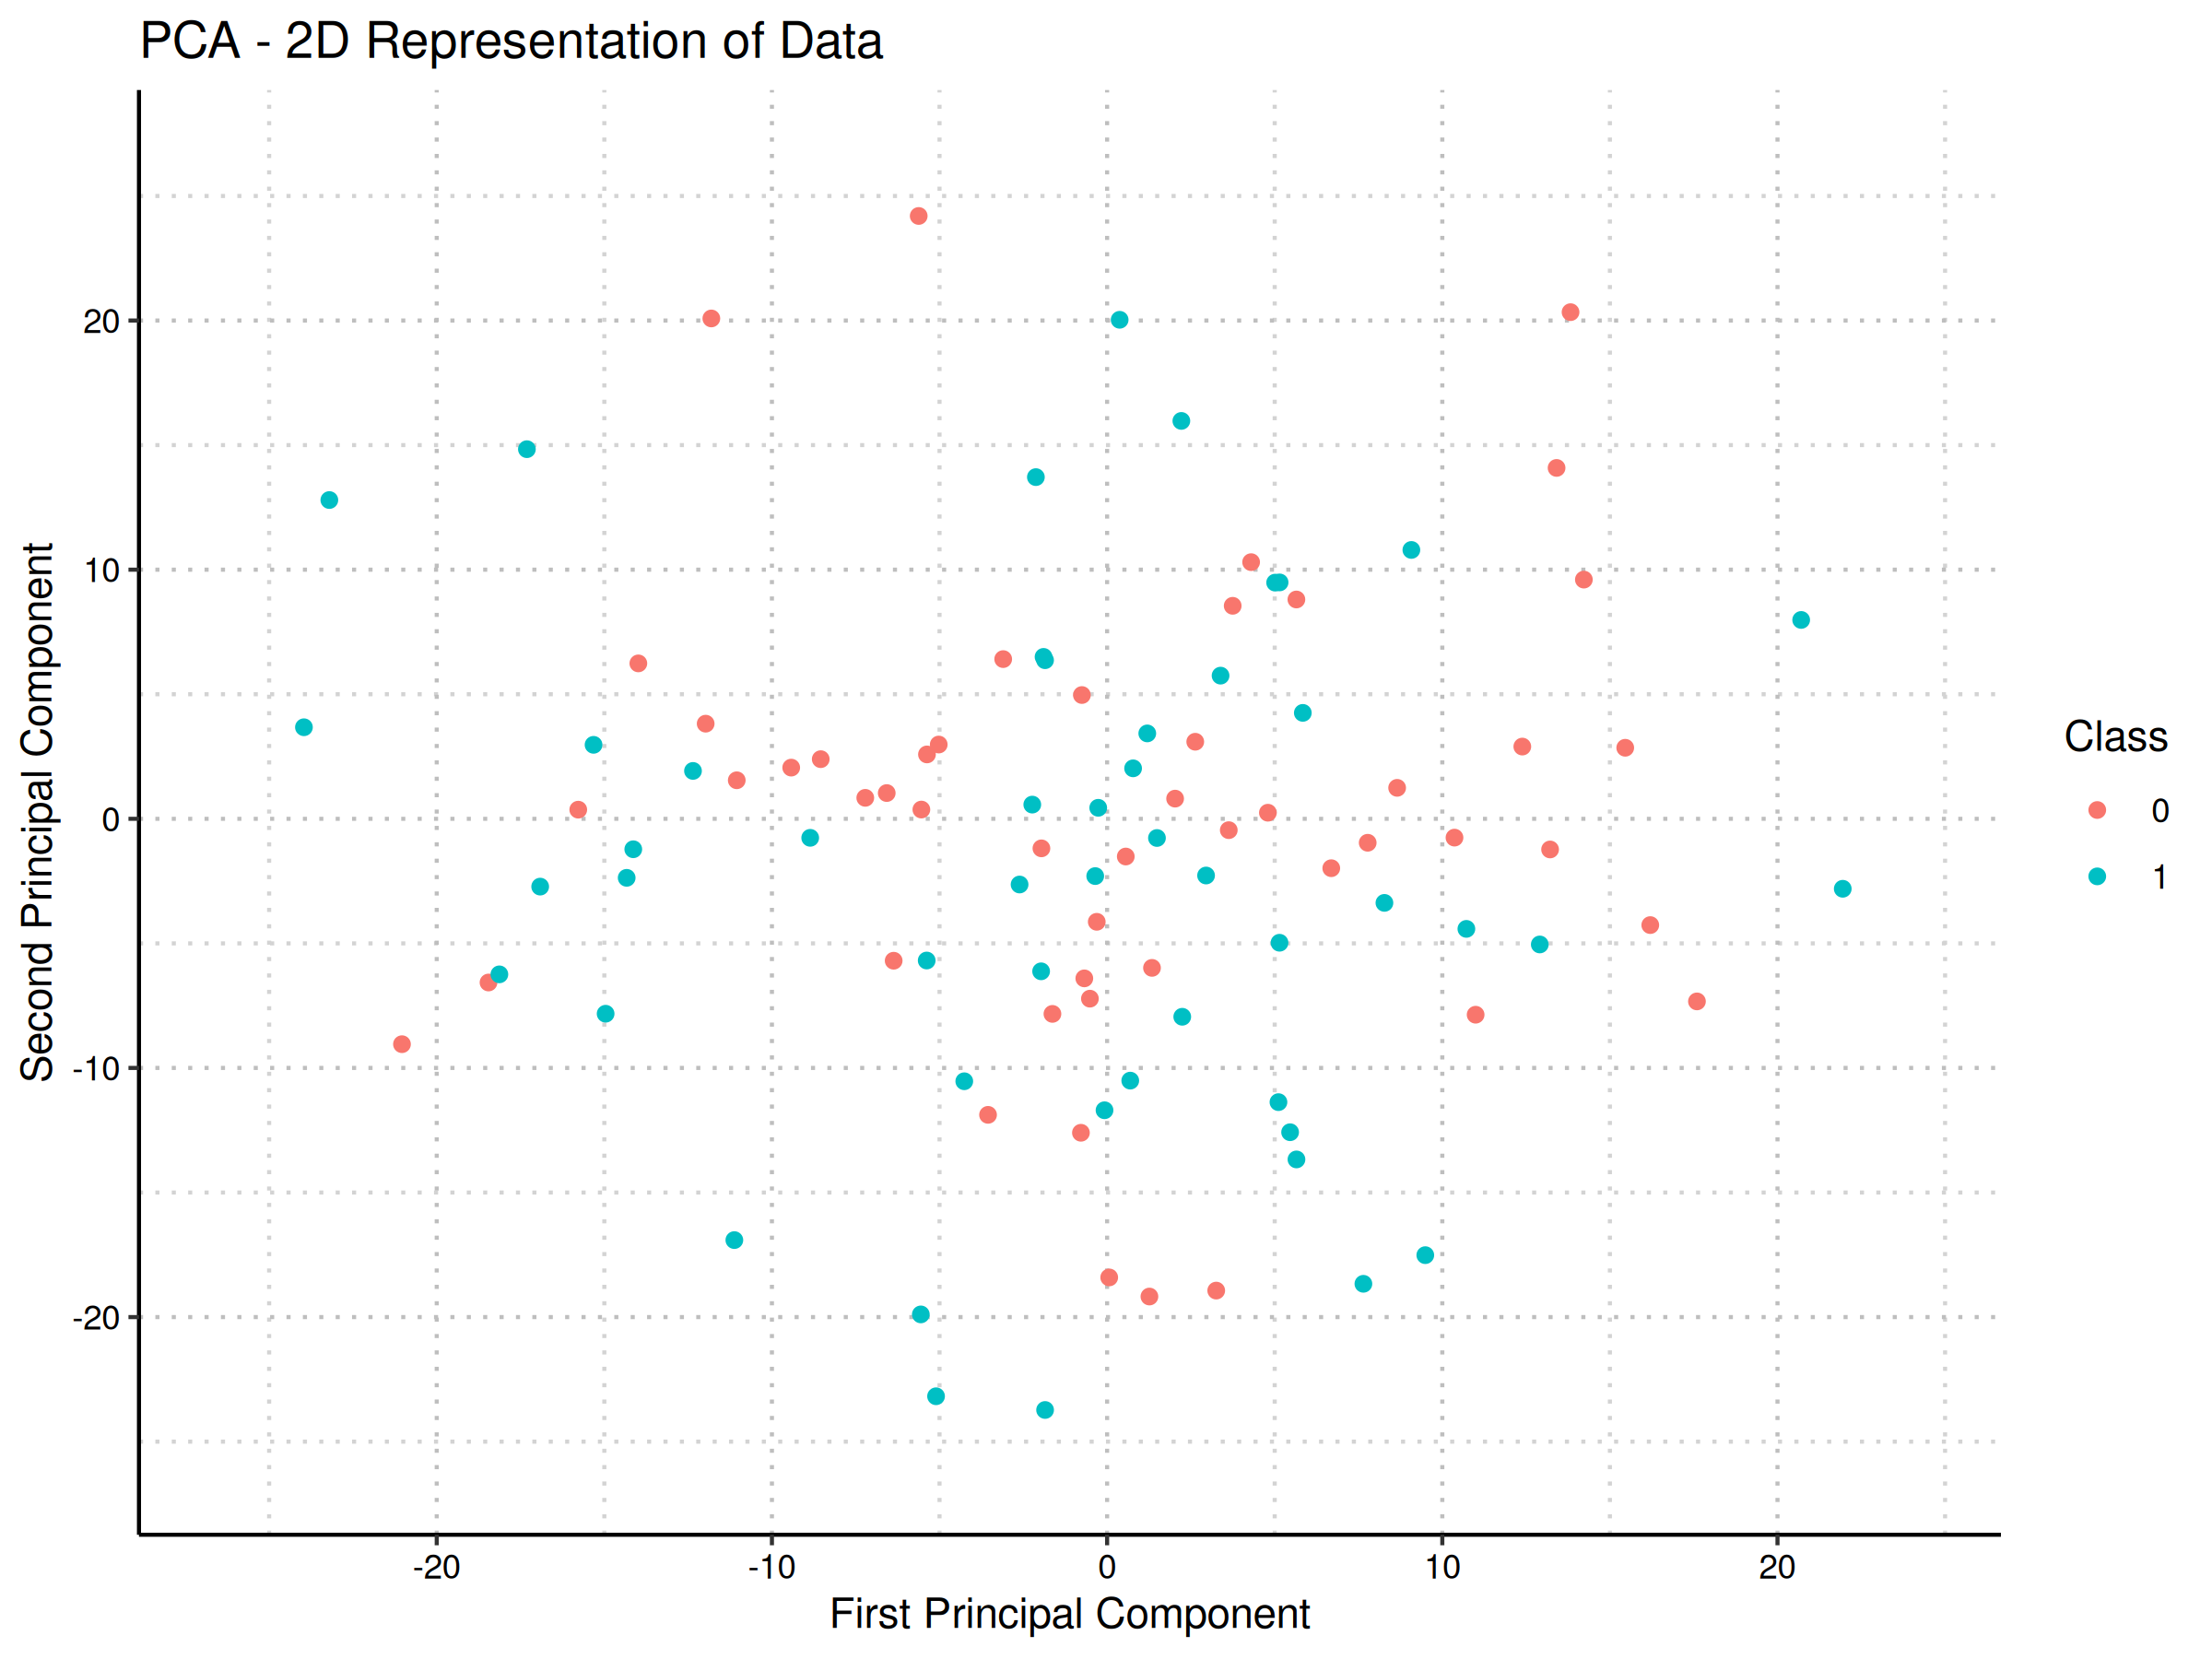
\includegraphics[scale = 0.5]{./images/clusters.png}
    \caption{Plane projection of the first two principal components of the explanatory variables simulated for 100 individuals when $\bm{\beta}_{\text{opti}}$ is given by the concatenation of pictograms in Fig: \ref{fig:picto_blocs}
    \label{fig:compos_plan}}
\end{figure}



\newpage

\section{Real dataset}

\subsection{Presentation of real data}

The actual data on which we are working comes from a cohort of 145 patients with liver tumors. 86 of them have CHC tumors, 22 have CCK tumors and 37 have mixed tumors. These proportions reflect the actual proportions of the different tumor classes in liver cancer patients. Each patient underwent four MRI radiographs of the liver, one at each time point after contrast injection. These were arterial, portal, venous and late. However, not all MRIs are usable. The patient may move during the MRI, rendering it unusable. A summary table (Table \ref{tab:nb_tumeurs}) is provided in order to specify the number of usable MRIs by temporality.\\
\indent Clinical data are also available: age at tumor detection, gender and patient alpha fetoprotein (AFP) levels. However, since the AFP levels of $22\%$ patients are missing from the data, we decided to exclude this clinical variable. As the gender of some patients (one with a CHC tumor, the other with a CCK tumor) was unknown, they were previously excluded from the study. The figures presented here and in the summary table Table \ref{tab:nb_tumeurs} show only those patients for whom we know the age at which the tumor was diagnosed and the gender.\\
\begin{table}[tbp]
    \centering
    \caption{Number of patients with usable MRI at the times indicated in the column for each tumor class. The total number of patients with each tumor class is entered in the total column.}
    \label{tab:nb_tumeurs}
    \begin{tabular}{|c|c|c|c|c|c|c|c|c|c|c|}
        \cline{1-7} \cline{9-9}
        class & Arterial & Portal & Venous & Late & All times & all times except venous& & total \\
        \cline{1-7} \cline{9-9}
        CHC & 84 & 81 & 83 & 78 & 72 & 74 & & 86\\
        \cline{1-7} \cline{9-9}
        CCK & 21 & 21 & 17 & 21 & 15 & 19 & & 22\\
        \cline{1-7} \cline{9-9}
        Mixtes & 35 & 36 & 32 & 34 & 29 & 31 & & 37\\
        \cline{1-7} \cline{9-9}
    \end{tabular}
\end{table}
\indent On each of the MRI, the tumor area is displayed and saved as a mask superimposed on the MRI. The MRIs and masks are in .nii format. Although taken at four different times, the four MRIs are very similar. In particular, the MRIs at venous and late time are extremely similar and often redundant in the eyes of radiologists. We'll take this opportunity to eliminate the venous time MRIs, as this is the time for which there are the most missing MRIs.
We propose two possible extractions for features. A 3D extraction, where features are extracted from the entire tumor volume, and a 2D extraction, where features are extracted from each tumor section. These extractions are the result of a calibration in which we used the performance of a lasso-penalized logistic model as a reference (to know which features to add or remove).\\
\indent As previously mentioned, we will only study the distinction between CHC and CCK tumors, which allows us to directly use the binary classification models described in the “Machine learning models” section.(\ref{sec:models}). 

\subsection{feature extraction in 3D}
\label{sec:3D}

We use the pyradiomics package \cite{pyradio} to extract an array of 3D features for each tumor. Only the original (unfiltered) image is used to extract these features. We extract all the first-order parameters (relative to gray levels), 3D shape parameters (volume, surface, etc.), and texture parameters (based on co-occurrence matrix, gradient matrix, etc.) proposed by the package (except those considered deprecated or duplicative: for example, we eliminate glcm joint average as it is redundant with glcm sum average). The result is $106$ features for each radio. Shape parameters are averaged over all extracted temporalities, as we consider that the shape of a tumor has no reason to change between different MRIs.\\
\indent The exact parameters used for pyradiomics extraction are given in appendix \ref{annexeparam}. They were recommended by ... . To ensure that the extraction is consistent from one tumor to the next, all tumors have been resampled to the same scale. On each $(x,y,z)$ axis, the spacing used is half the median spacing on that axis (calculated over all available MRIs). The idea behind this spaing is to avoid losing too much information by increasing the voxel size of higher-resolution MRIs without having to completely interpolate lower-resolution MRIs. Image interpolations are performed using cubic splines, while mask interpolations are based on the closest interpolation method (to guarantee mask connectivity).\\

\subsection{Feature extraction in 2D}
\label{sec:2D}
The first step in this extraction process is to determine the slices we wish to extract from your tumour. We choose the axial plane for the slices, as this is the one used by radiologists when analyzing a tumor. As for the extraction parameters, they are again given in Appendix \ref{annexeparam}. However, we can't simply extract slices at regular intervals along the vertical axis, for two reasons:\\
\indent Firstly, tumor size varies from patient to patient. Thus, a certain spacing between slices will lead to the extraction of 3 slices of tumors in some patients and 10 slices in others. However, the machine learning models we use need to compare the same features in all patients. Secondly, slices with a very small piece of tumor are not very significant for our analysis. However, extracting at regular intervals will lead to the extraction of such slices at the beginning and end of certain elongated tumors (along vertical axis). We'd therefore like to give more importance to slices where the tumor is most present (without completely ignoring slices with less tumor on them).\\
\indent We therefore propose an extraction where we first specify the number of slices $n_{\text{slices}}$ to be extracted from each tumor. We begin by interpolating the cumulative distribution of tumor volume by depth (along the vertical axis) for each tumor (see Fig. \ref{fig:depth_volume}). This curve is then inverted to obtain the depth distribution as a function of the cumulative tumour volume covered. A slice is then extracted at each of the following depths: 
\begin{equation}
(i-0.5) \displaystyle{\frac{\text{area}_{\text{max}}}{n_{\text{slices}}}} \hspace{1.5 cm} \text{for i } \in \llbracket 1,n_{\text{slices}}  \rrbracket
\end{equation}
We have tried other extraction methods, in particular trying to extract precisely the same depths for each MRI of the same tumor, and taking into account the fact that the patient may have moved slightly between two MRIs. However, as the results were of lesser quality, we will not develop these approaches here.\\
\indent The features extraction used for each slice is almost the same as the one used for the 3D tumor (in the previous section), except for shape parameters. In fact, 2D shape parameters (instead of 3D shape parameters) are now extracted. 2D shape parameters are always averaged over all MRIs of the same tumor (variations in tumor shape between MRIs result solely from changes in the way radiologists cut masks, and therefore do not provide information on the tumor itself).\\

\begin{figure}[tbp]
    \centering
    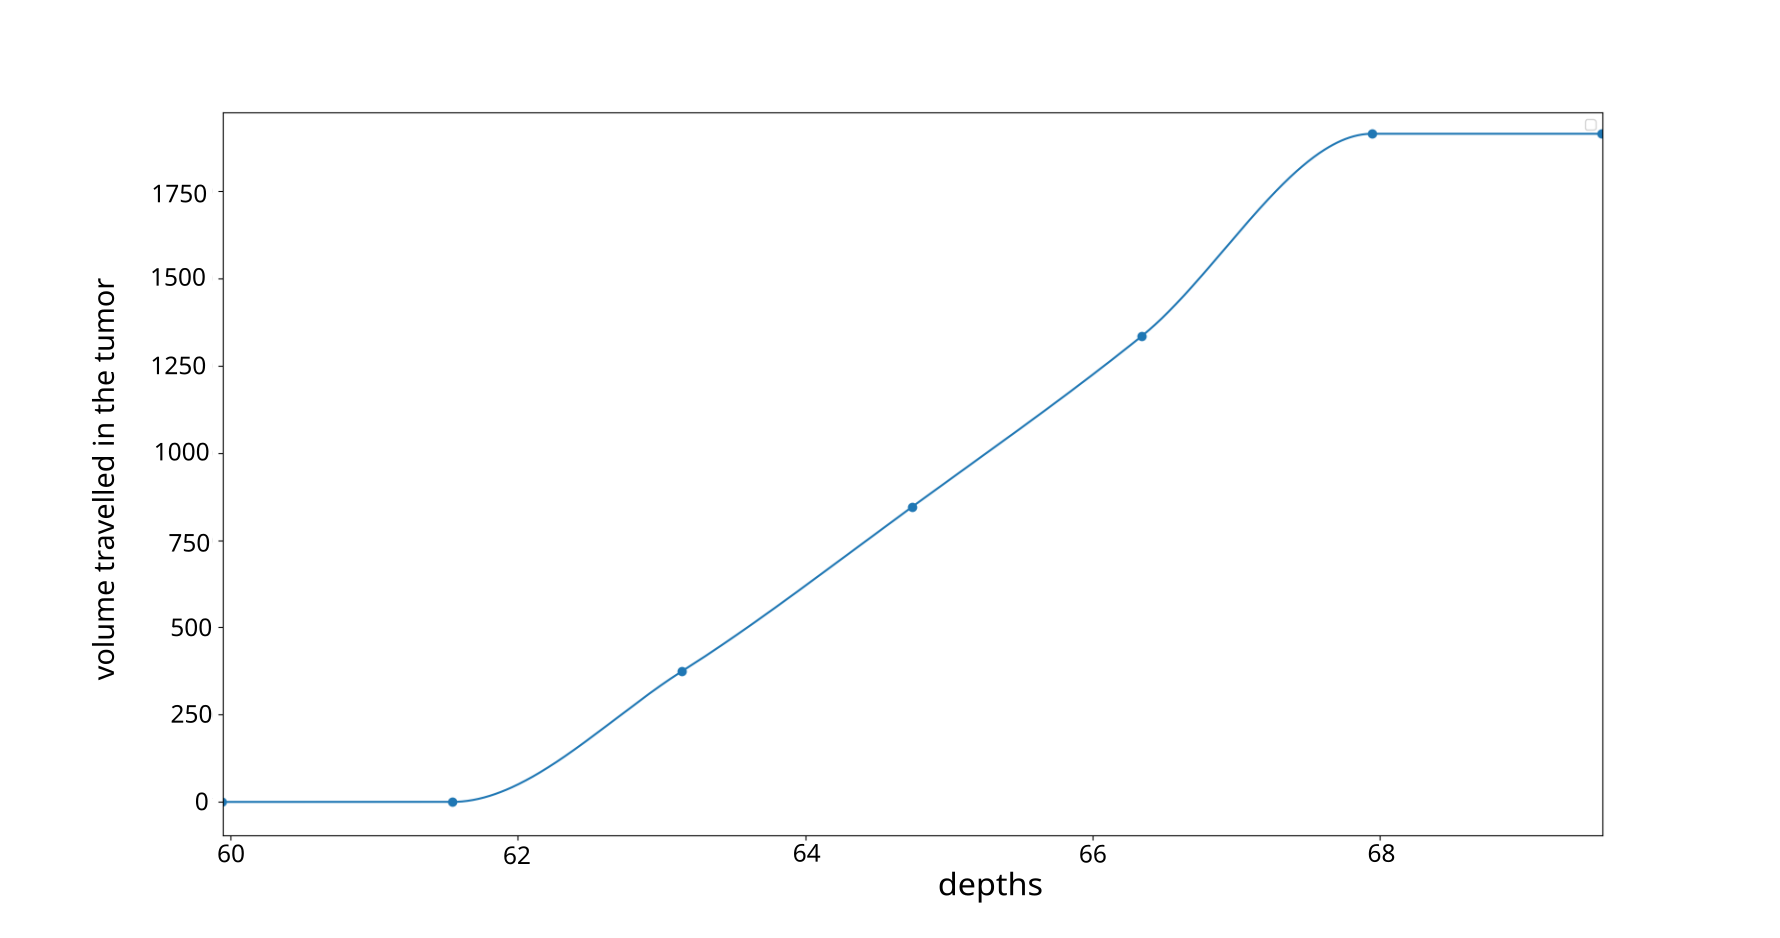
\includegraphics[scale = 0.25]{./images/plot_depth_volume_2.png}
    \caption{graph of the cumulative volume distribution (in $mm^3$) of the third CCK patient's tumor according to depth (in $mm$) for a given tumor. The points correspond to the slices recorded in the sitk image (with its initial spacing). The curve is obtained by interpolating these points using Hermite cubic splines.}
    \label{fig:depth_volume}
\end{figure}

\subsection{Extraction of healthy liver parts}
We wanted to add the features obtained by performing the extraction on portions of healthy liver. Radiologists generally compare the luminosity of the tumor area with the rest of the liver, so it seemed appropriate to do the same with our model.\\
\indent To do this, a small strip of tissue was extracted around the tumor area. To ensure that no area outside the liver or crossed by a blood vessel was included, we decided to extract only areas of low local variance and whose luminosity was greater than that of the black background. By adding a 3D connectivity criterion, we can extract a 3D area of healthy liver large enough to perform a 3D extraction of firstorder and texture features (the shape of the extracted area being of no interest).\\
\indent To ensure that the same area of healthy tissue was extracted from each MRI of the same tumour, we decided to crop the healthy tissue on the late MRI only (this was when our extraction method was most visually successful). We then applied the same trimming to the other MRIs, shifting the extracted area slightly to take account of the patient's movements. These movements were estimated by comparing the tumor areas on each slice and trying to increase as much as possible the intercorrelation of the area curves between each MRI and the late MRI. This procedure is performed along all three spatial axes. Finally, the extracted zone can be visualized, as in Fig. \ref{fig:healthy_zone} to check that the extraction is proceeding correctly.\\
\indent However, we did not perceive any improvement in the performance of our models by adding these features. We therefore decided not to include them in the rest of our study.\\

\begin{figure}[tbp]
    \centering
    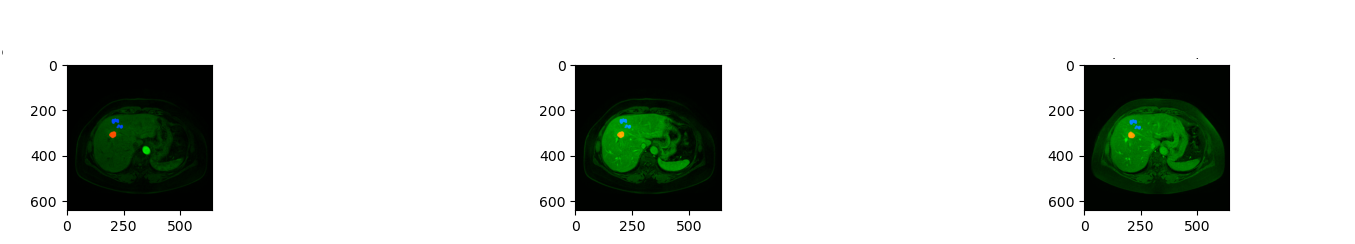
\includegraphics[scale = 0.3]{./images/sain.png}
    \caption{MRIs of a CCK tumor slice with the tumor area in red and the peripheral area of extracted healthy liver in blue. From left to right, arterial, portal and late MRIs. Axes are graduated in mm.}
    \label{fig:healthy_zone}
\end{figure}

\newpage
\section{results}
\label{sec:results}
\subsection{Simulated data}

We performed tests on simulated data generated with the parameters presented in \ref{annexe:hyperparam}. The pictogram to retrieve is the one in figure \ref{fig:picto_blocs}. We evaluated the performance in two settings: one with a lot of individuals to classify ($3000$ individuals in the training data set) and another with fewer individuals to classify ($500$ individuals in the training dataset). The testing dataset is always composed of $1000$ individuals. We consider the area under curve to determine the performance of each model as it is a robust and fine grained indicator of the efficience of each model to separate the two classes. We show the results in Table \ref{tab:result_simul}. Pour chaque modèle, les hyperparamètres utilisés lors de la cross validation sont fournis en \ref{annexe:hyperparam}. On présente dans chaque cas le pictogramme reconstruit en \ref{annexe:picto}\\
\indent On constate qu'en présence d'un grand nombre d'individus (3000 individus), le modèle multiway multibloc réussit le mieux à reconstutuer les pictogrammes. En terme de performance, mesurée par l'area under curve, il ses performances dans ce paramétrage sont similaires à celles du modèle multiway. Les autres modèles (group lasso et régression logistique classique avec lasso) sont largement moins performants qu les deux modèles tensoriels.
En présence d'un faible nombre d'individus (500 individus) c'est cete fois-ci le modèle multiway qui est le plus performant. En effet, il permet de capturer en un très faible nombre de paramètres la structure des pictogrammes (le rang choisi par la cross validation est égal à 1 des cette configuration). Même en imposant un rang égal à 1 au modèle multiway multibloc, celui-ci nécessite le calcul de davantage de coefficients (environ $2$ fois plus dans le cas de nos pictogrammes), ce qui peut conduire à une plus forte surinterprétation.\\
\indent Ces simulations démontrent bien l'utilité des modèles tensoriels pour la classification de données de haute dimension. Cependant, même si elles montrent que la structure du coefficient $\beta$ est plus facilement retrouvé par le modèle multiway multibloc (quand $\beta$ a une structure par bloc, comme c'est le cas pour nos pictogrammes), elles n'indiquent pas de surperformance en classification du modèle multibloc par rapport au modèle multiway.\\

\begin{table}[tbp]
    \centering
    \caption{Area under curve for each model. For the group lasso model, it is possible to group variables by bloc, mode or variable. On indique entre parenthèses quel type de groupement a été utilisé.}
    \label{tab:result_simul}
    \renewcommand{\arraystretch}{1.2} 
    \begin{adjustbox}{center}
    \begin{tabular}{|>{\centering\arraybackslash}m{2cm}|>{\centering\arraybackslash}m{2.5cm}|>{\centering\arraybackslash}m{2.5cm}|>{\centering\arraybackslash}m{2.5cm}|>{\centering\arraybackslash}m{2.5cm}|>{\centering\arraybackslash}m{2cm}|>{\centering\arraybackslash}m{2.5cm}|}
        \cline{1-7}
        number of individuals & lasso & goup lasso (by bloc) & goup lasso (by mode)& group lasso (by variable) & multiway & multiway multibloc\\
        \cline{1-7} 
        3000 & 0.83 & 0.86 & 0.94 & 0.94 & 0.99 & 0.99 \\
        \cline{1-7}
        500 & 0.59 & 0.65 & 0.64 & 0.63 & 0.92 & 0.63 \\
        \cline{1-7}
    \end{tabular}
\end{adjustbox}
\end{table}

\subsection{real data}
\indent Nous avons réalisé des tests sur les données simulées d'une part en utilisant les features 3D exclusivement (comme décrit dans \ref{sec:3D}) et d'autre part en utilisant les features 2D (comme décrit dans \ref{sec:2D}). Les résultats sont présentés pour chaque model dans le tableau \ref{tab:result_real}. Tous les résulats sont moyennés sur $50$ entraînements différents. On propose assi une analyse de l'importance de chaque feature des données étudiées.\\
\indent On mesure l'importance d'une feature comme la valeur absolue du coefficient $\beta$ qui se trouve devant elle. Il suffit ensuite de moyenner cette valeur sur tous les entraînements pour trouver l'importance de la feature. Etant donné le grand nombre de features, on les regroupe par bloc, mode et/ou nom de variable. L'importance d'un bloc est donnée comme la somme des importances de ses features. Toutes les importances sont finalement renormalisées pour que leur somme fasse $1$ (on s'intéresse à l'importance relative des features les unes par rapport aux autres). On donne en \ref{annexe:importance} les graphes des importances relatives des features dans chaque modalité d'entraînement (données 2D ou 3D) pour le modèle le plus performant (group lasso pour les données 3D et ... pour les données 2D).\\
\begin{table}[tbp]
    \centering
    \caption{Moyenne des area under curve obtenues avec chaque model pour 50 entrainements différents (avec une partition différente entre training set et testing set). For the group lasso model, it is possible to group variables by bloc, mode or variable. On indique entre parenthèses quel type de groupement a été utilisé.}
    \label{tab:result_real}
    \renewcommand{\arraystretch}{1.2} 
    \begin{adjustbox}{center}
    \begin{tabular}{|>{\centering\arraybackslash}m{2cm}|>{\centering\arraybackslash}m{2.5cm}|>{\centering\arraybackslash}m{2.5cm}|>{\centering\arraybackslash}m{2.5cm}|>{\centering\arraybackslash}m{2.5cm}|>{\centering\arraybackslash}m{2cm}|>{\centering\arraybackslash}m{2.5cm}|}
        \cline{1-7}
        Type of data & lasso & goup lasso (by bloc) & goup lasso (by mode)& group lasso (by variable) & multiway & multiway multibloc\\
        \cline{1-7} 
        3D & 0.74 & 0.78 & 0.76 & 0.73 & 0.77 & xxx \\
        \cline{1-7}
        2D & xxx & xxx & xxx & xxx & xxx & xxx \\
        \cline{1-7}
    \end{tabular}
\end{adjustbox}
\end{table}

\section{Conclusion de l'article}



%% The Appendices part is started with the command \appendix;
%% appendix sections are then done as normal sections

%% For citations use: 
%%       \cite{<label>} ==> [1]

%%

%% If you have bib database file and want bibtex to generate the
%% bibitems, please use
%%
\newpage
 \bibliographystyle{elsarticle-num} 
 \bibliography{bibliography.bib}

%% else use the following coding to input the bibitems directly in the
%% TeX file.

%% Refer following link for more details about bibliography and citations.
%% https://en.wikibooks.org/wiki/LaTeX/Bibliography_Management

\newpage

\appendix

\section{Pseudo-code for multiblock multivariate logistic regression with lasso}
\label{annexecode}

In order to be more readable, we keep the notations that were used during the presentation of the model.\\[5 pt]

\begin{mdframed}[leftmargin=0cm, rightmargin=4cm]
    \noindent \textbf{Inputs}\\
    \phantom{a}\hspace{5 pt} $\bullet$ $\epsilon >0$, $\lambda >0$, $R \in \mathbb{N}^{*}$\\[2 pt]
    \phantom{a}\hspace{5 pt} $\bullet$ $\bm{\beta}^{K(0)} \in \mathbb{R}^{LRK}$\\[4 pt]
    \textbf{Treatment}\\
    \phantom{a}\hspace{5 pt} $\bullet$ $q \leftarrow 0$\\[2 pt]
    \phantom{a}\hspace{5 pt}  \textbf{Repeat}\\[2 pt]
    \begin{tikzpicture}[overlay, remember picture]
        \draw[thick] (0.9, 0.18) -- (0.9, -3.75);  % Modifier les coordonnées pour ajuster la position et la
    \end{tikzpicture}
    \phantom{a}\hspace{22 pt} $\bullet$ Construct $\mathbf{Z}^J$ according to \cref{eqref: Z_j,eqref: Z_r}\\[2 pt]
    \phantom{a}\hspace{25 pt} $\bullet$ Construct $\mathbf{Q}^J$ according to \cref{eqref:Q^J}\\[2 pt]
    \phantom{a}\hspace{25 pt}  $\bullet$ $(\beta_0^{(q)}, \bm{\beta}^{J {(q)}}) \longleftarrow \hspace{-10 pt} \underset{(\beta_0, \bm{\beta}) \in \mathbb{R} \times \mathbb{R}^{RJ + M}}{\text{argmin}} \left( C(\beta_0, (\mathbf{Q}^J)^{-1}\bm{\beta},\mathbf{Z}^J \mathbf{Q}^J, \mathbf{y}, \lambda) \right)$\\[2 pt]
    \phantom{a}\hspace{25 pt} $\bullet$ Construct $\mathbf{Z}^K$ according to \cref{eqref: Z^K,eqref: Z_tens^K}\\[3 pt]
    \phantom{a}\hspace{25 pt} $\bullet$ Construct $\mathbf{Q}^K$ by adapting \cref{eqref:Q^J}\\[2 pt]
    \phantom{a}\hspace{25 pt}  $\bullet$ $(\beta_0^{(q)}, \bm{\beta}^{K {(q)}}) \longleftarrow \hspace{-10 pt} \underset{(\beta_0, \bm{\beta}) \in \mathbb{R} \times \mathbb{R}^{LRK + M}}{\text{argmin}} \left( C(\beta_0, (\mathbf{Q}^K)^{-1}\bm{\beta},\mathbf{Z}^K \mathbf{Q}^K, \mathbf{y}, \lambda) \right)$\\[2 pt]
    \phantom{a}\hspace{25 pt}  $\bullet$ $q \leftarrow q + 1$\\[4 pt]
    \phantom{a}\hspace{8 pt}  \textbf{until} $|C^K - C^J| < \epsilon |C^J| $\\[4 pt]
    \textbf{Return} $(\beta_0^{(q)},\bm{\beta}^{K(q)}, \bm{\beta}^{J(q)})$
\end{mdframed}

\newpage

\section{Hyperparameters for simulated data}
\label{annexe:hyperparam}
\subsection{Data generation}

\noindent In our simulations, we unfold the $\beta^l$ of each pictogram line by line into a vector (rather than a matrix) and concatenate these vectors to obtain $\bm{\beta} = [\bm{\beta}^1; \; \hdots \; \bm{\beta}^L]$. Let $N$ be the size of $\bm{\beta}$. We then use the following parameters to generate the simulated data:
\begin{itemize}[label = $\bullet$]
    \item $\bm{\mu}_0 = \mathbb{0}_N$
    \item $\bm{\mu}_1 = \bm{\beta}/\lVert \bm{\beta}\rVert$ 
    \item $\mathbf{P}$ is obtained by completing in orthonormal basis $\bm{\beta}/\lVert \bm{\beta}\rVert$
    \item $d_1 = 0.01$
    \item For $i \in \llbracket 2, N \rrbracket$, $d_i = 0.25$ (where ($d_i$) are the diagonal elements of $\mathbf{D}$) 
\end{itemize}

On $1000$ individuals generated, with 500 in each class, the accuracy obtained by the 2-means algorithm is $0.48$: in other words, it doesn't do better than chance (even slightly worse in our case). However, the section \ref{sec:results} shows far better performance from our models

\subsection{Cross validation of models}

\noindent Pour les modèles lasso et group lasso, on cross-valide sur $20$ valeurs de $\lambda$ réparties selon une échelle logarithmique entre $10^{-5}$ et $10^{-13}$.\\
\indent Pour le modèle muliway et le modèle multiway mulibloc, on cross valide sur $5$ valeurs de $\lambda$ réparties selon une échelle logarithmique entre $10^{-3}$ et $10^{-6}$. On cross valide aussi sur le rang utilisé. Le rang de $\bm{\beta}_{\text{opti}}$ est majoré par la somme des rangs des pictogrammes individuels (respectivement environ $15$, $1$ et $10$). On ne dépassera donc pas $27$ pour rang dans notre cross validation. On espère en fait approximer $\beta$ avec une matrice de rang inférieur à $26$ pour assurer une certaine sparsité dans le modèle. On cross-valide donc sur les rangs $1$, $10$ et $20$ dans le modèle multiway (pour proposer un paramétrage du modèle avec un rang minimal, un rang intermédiaire et un rang élevé).\\
\indent Dans le modèle multibloc, on a la possibilité de choisir un rang pour chaque pictogramme. Afin de ne pas surcharger la cross validation, on se limite à cross-valider sur le rang du premier pictogramme. En effet, il s'agit du pictogramme de rang le plus élevé et il y a donc plus de "choix" différents possibles pour le modèle multibloc, selon la sparsité souhaitée. On propose donc les rangs $1$, $6$ et $12$ pour ce pictogramme dans la cross validation. Pour les autres pictogrammes, on impose respectivement $1$ et $10$. Là encore, on cross valide aussi sur $5$ valeurs de $\lambda$, réparties selon une échelle logarithmique entre $10^{-3}$ et $10^{-6}$.





\newpage

\section{Parameters used for feature extraction with pyradiomics}
\label{annexeparam}

List of parameters used for feature extraction by pyradiomics:
 
\begin{itemize}[label = $\bullet$]
    \item Bin width : 25
    \item Resampled Pixel Spacing : $[2,2,2]$ si l'extraction est en 3D, $[2,2]$ si elle est en 2D
    \item interpolator : sitkBSpline
    \item force2D : True
    \item force2Ddimension : 2
\end{itemize}


\section{Reconstructed pictograms}
\label{annexe:picto}

\begin{figure}[H]
    \centering
    \begin{tabular}{cc}
        \subfloat[lasso \label{fig:3000simple}]{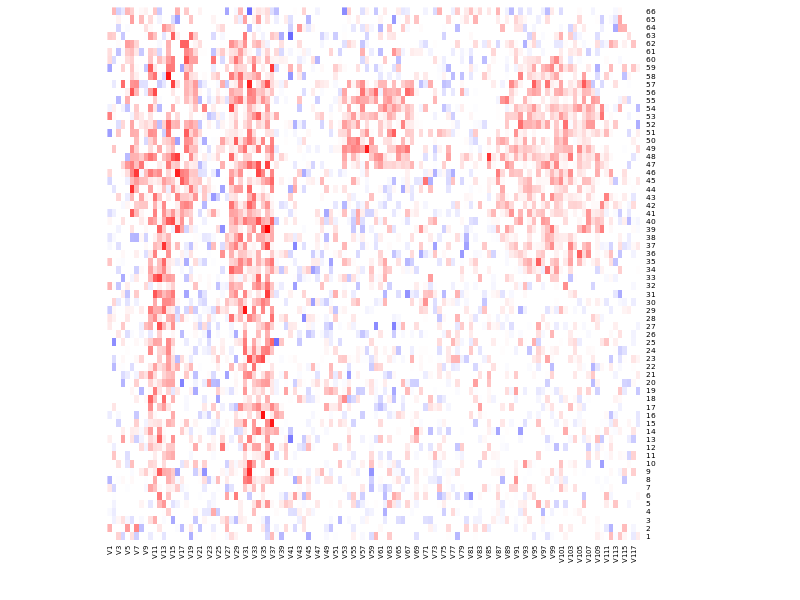
\includegraphics[width=0.35\textwidth]{images/heatmap_logistique_simple_simu_4000.png}} &
        \subfloat[group lasso (bloc)\label{fig:3000bloc}]{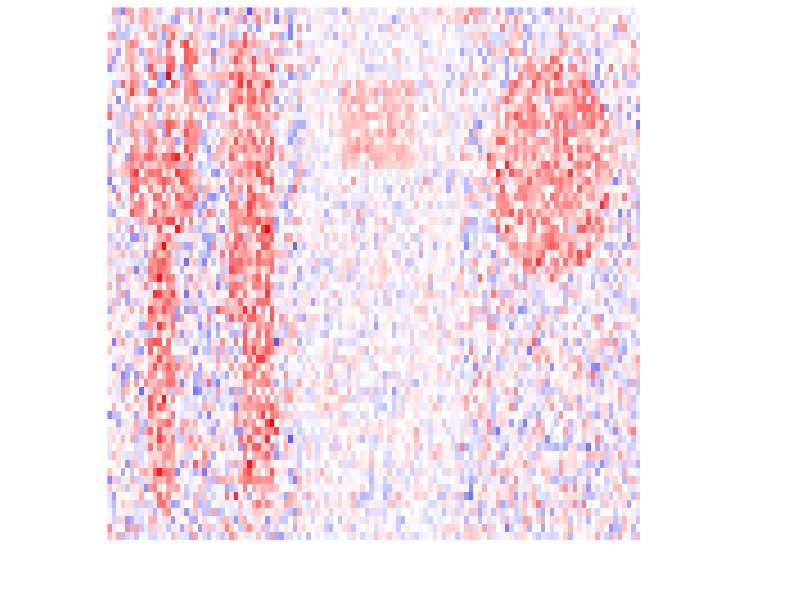
\includegraphics[width=0.35\textwidth]{images/heatmap_logistic_grp_simu_4000_bloc.png}} \\
        \subfloat[group lasso (variable)\label{fig:3000var}]{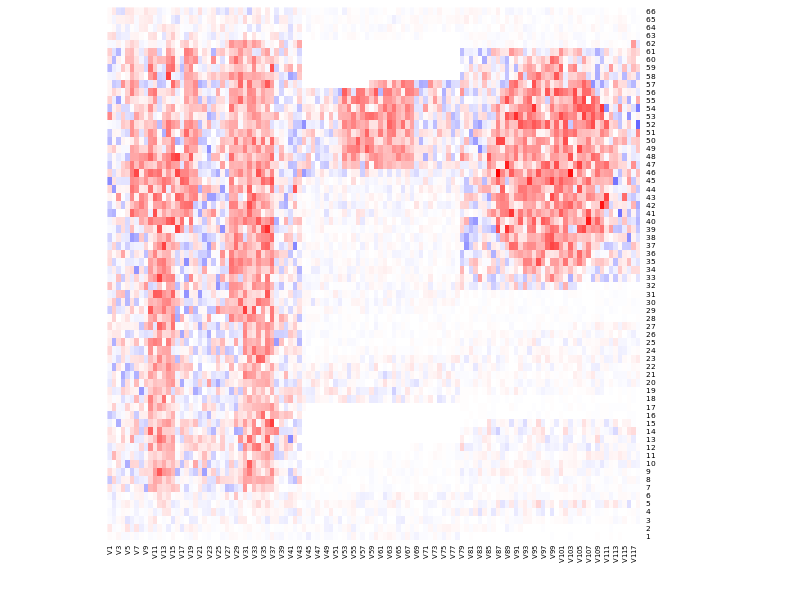
\includegraphics[width=0.35\textwidth]{images/heatmap_logistic_grp_simu_4000_var.png}} &
        \subfloat[group lasso (mode)\label{fig:3000mode}]{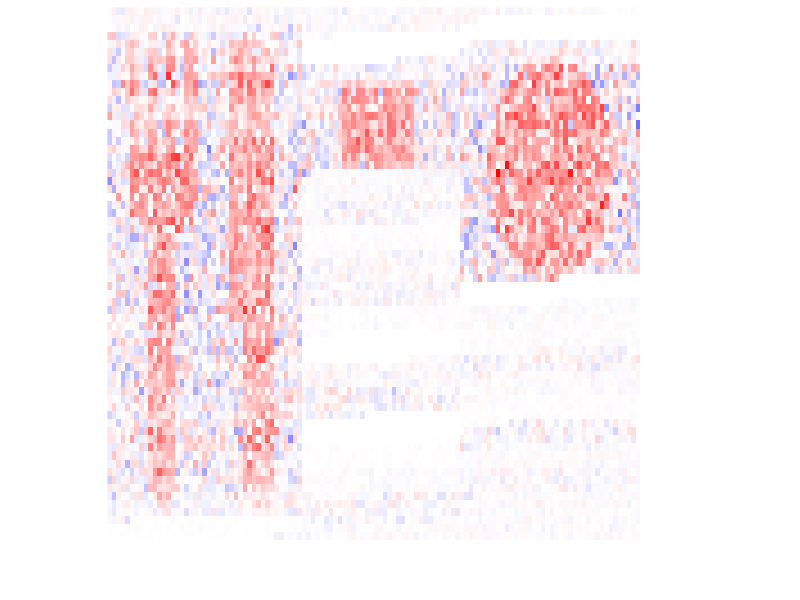
\includegraphics[width=0.35\textwidth]{images/heatmap_logistic_grp_simu_4000_mode.png}} \\
        \subfloat[multiway\label{fig:3000multiway}]{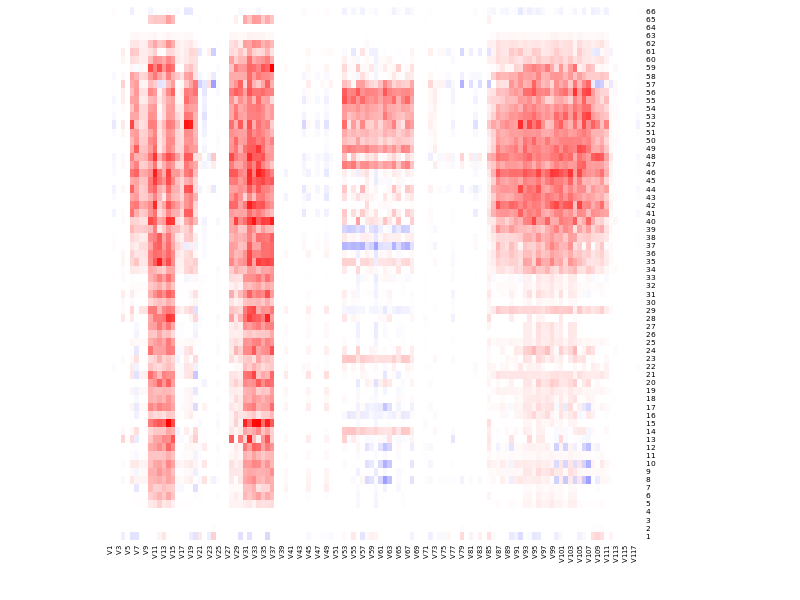
\includegraphics[width=0.35\textwidth]{images/heatmap_logistic_multibloc_simu_4000_multiway.png}} &
        \subfloat[multiway multibloc\label{fig:3000multibloc}]{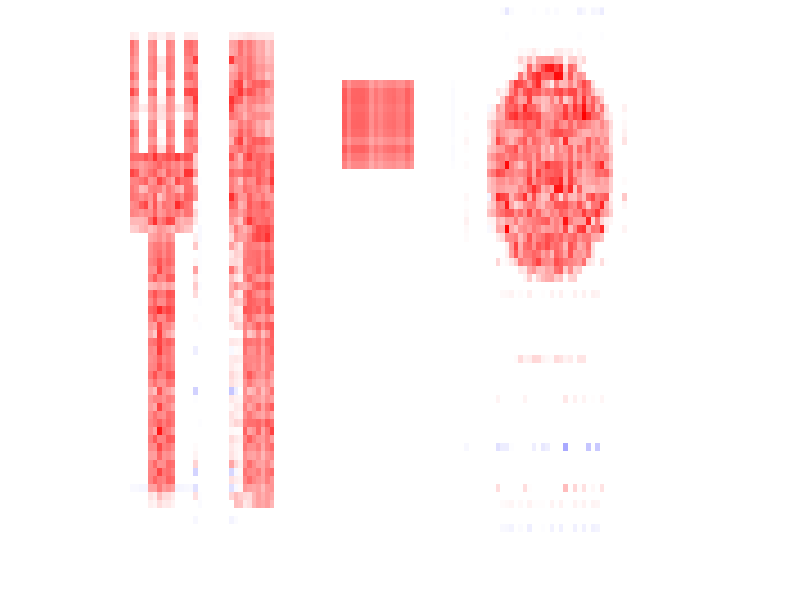
\includegraphics[width=0.35\textwidth]{images/heatmap_logistic_multibloc_simu_4000.png}} \\
    \end{tabular}
    \caption{Pictogrammes reconstruits par les différents modèles pour $3000$ individus dans le training dataset. Le nom du modèle utilisé est indiqué dans la légende de chaque figure.}
    \label{fig:tableau_figures_3000}
\end{figure}

\begin{figure}[H]
    \centering
    \begin{tabular}{cc}
        \subfloat[lasso \label{fig:500simple}]{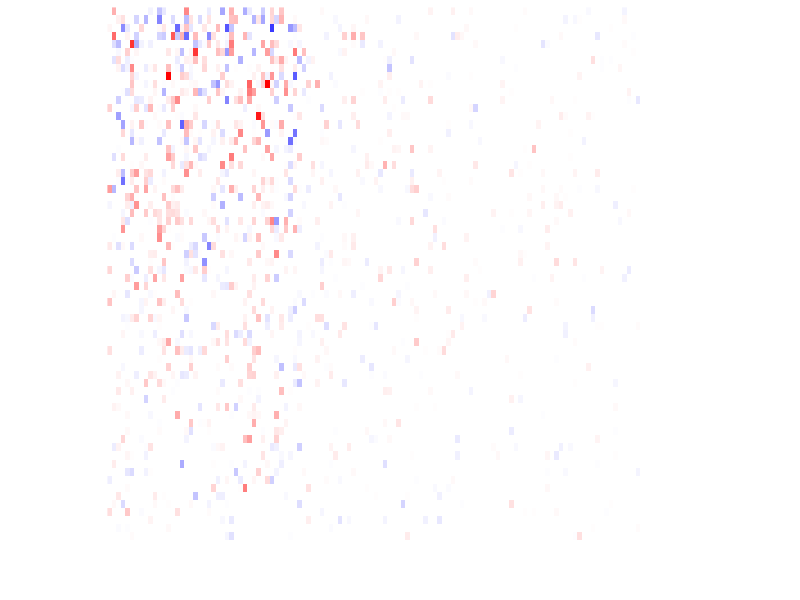
\includegraphics[width=0.35\textwidth]{images/picto_500/heatmap_logistique_simple_simu_500.png}} &
        \subfloat[group lasso (bloc)\label{fig:500bloc}]{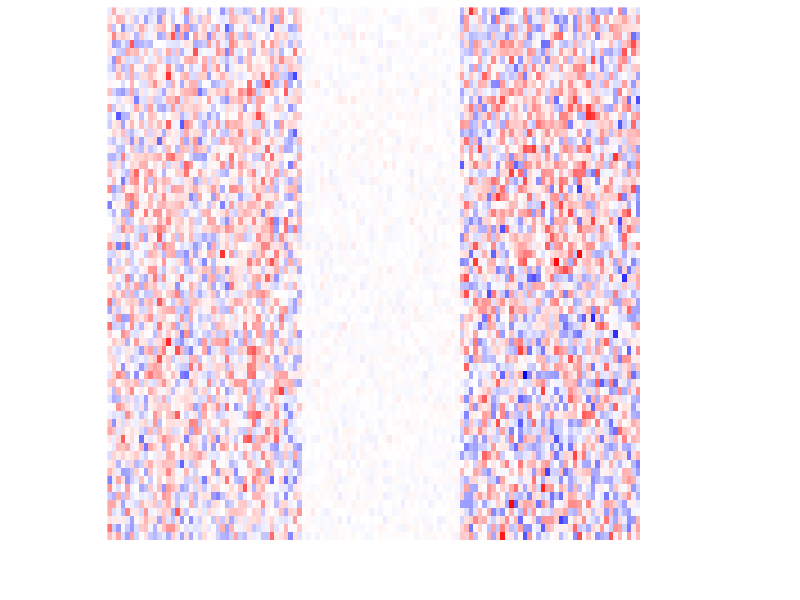
\includegraphics[width=0.35\textwidth]{images/picto_500/heatmap_logistic_grp_simu_500_bloc.png}} \\
        \subfloat[group lasso (variable)\label{fig:500var}]{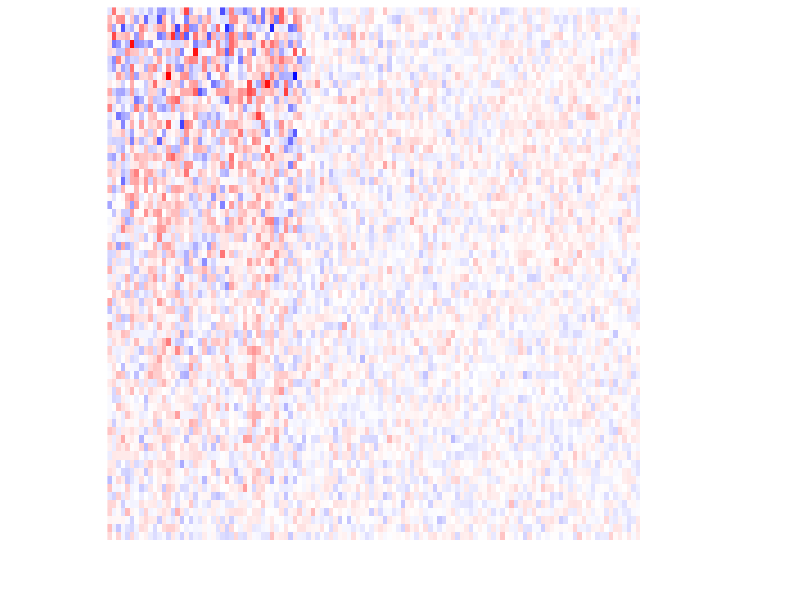
\includegraphics[width=0.35\textwidth]{images/picto_500/heatmap_logistic_grp_simu_500_var.png}} &
        \subfloat[group lasso (mode)\label{fig:500mode}]{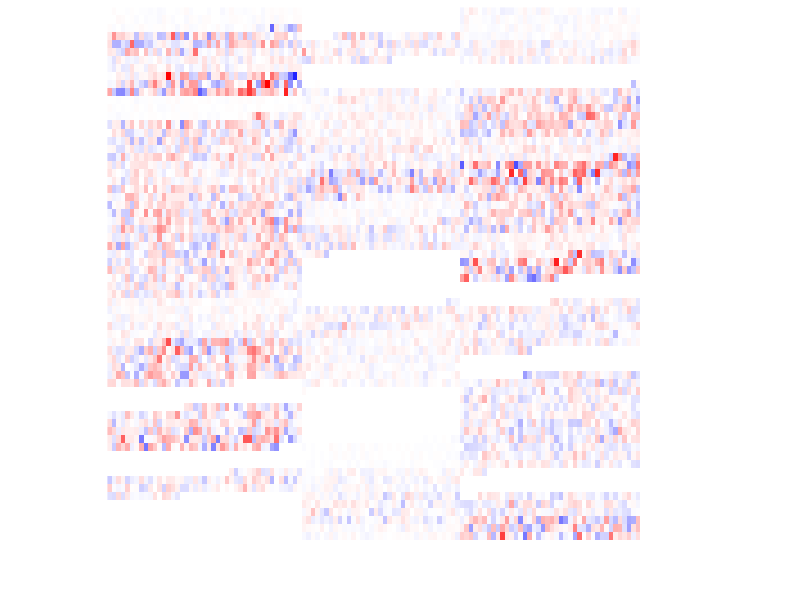
\includegraphics[width=0.35\textwidth]{images/picto_500/heatmap_logistic_grp_simu_500_mode.png}} \\
        \subfloat[multiway\label{fig:500multiway}]{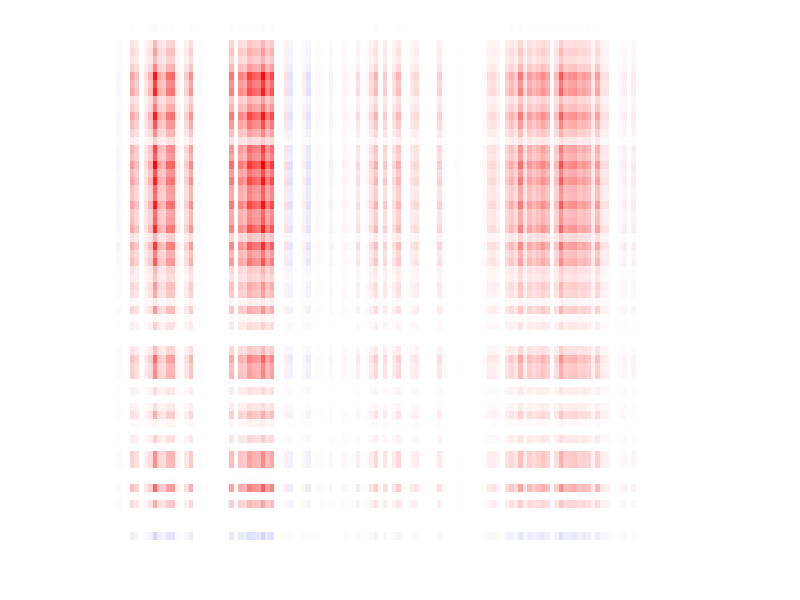
\includegraphics[width=0.35\textwidth]{images/picto_500/heatmap_logistic_multibloc_simu_500_multiway.png}} &
        \subfloat[multiway multibloc\label{fig:500multibloc}]{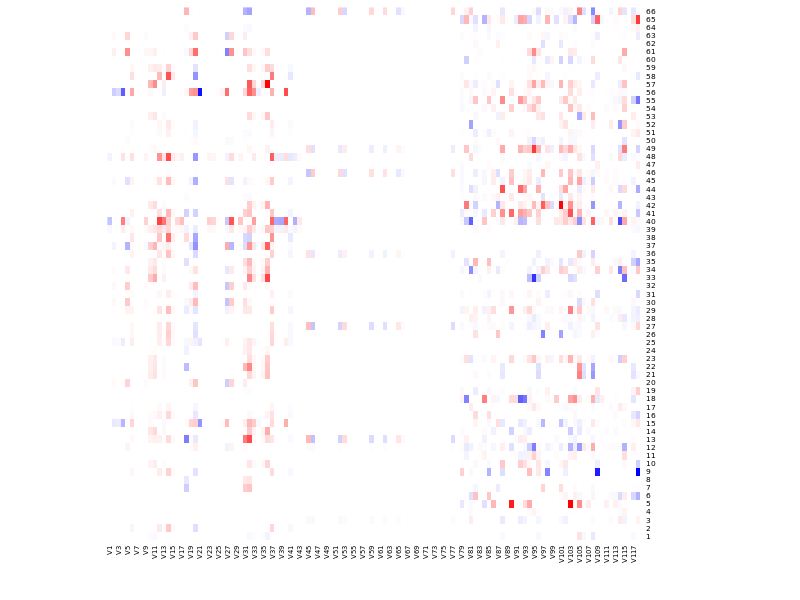
\includegraphics[width=0.35\textwidth]{images/picto_500/heatmap_logistic_multibloc_simu_500.png}} \\
    \end{tabular}
    \caption{Pictogrammes reconstruits par les différents modèles pour $500$ individus dans le training dataset. Le nom du modèle utilisé est indiqué dans la légende de chaque figure.}
    \label{fig:tableau_figures_500}
\end{figure}

\newpage 
\section{Importance of features}
\label{annexe:importance}
\noindent On donne ici les graphes d'importance des modèles les plus performants (en terme d'AUC, cf Table \ref{tab:result_real}), à savoir le modèle group lasso pour les données 3D et le modèle ... pour les données 2D.\\
\indent Sur chaque bâton de chaque diagramme en bâtons, on peut lire un pourcentage en vert. Celui-ci renseigne sur le nombre de fois où le coefficient devant les features associées au bâton a été non nul. En effet, tous nos modèles étant pénalisés au lasso, ils tendent à mettre à zéro les coefficients des variables les moins importantes. On peut donc calculer pour chaque variable, sur les $50$ entraînements effectués, le pourcentage de fois où ce coefficient a été non nul. La moyenne de ces pourcentages sur toutes les features d'un groupe de features (bloc, mode ou variable) est indiqué en vert sur le graphe. Cette moyenne reflète le nombre de fois où les features de ce groupe ont été jugées importantes par le modèle (i.e. leur coefficient de régression a été non nul).\\

\end{document}

\endinput
%%
%% End of file `elsarticle-template-num.tex'.
